\documentclass[12pt,a4paper]{report}

% Packages
\usepackage{geometry}
\usepackage{amsmath}
\usepackage{amsfonts}
\usepackage{amssymb}
\usepackage{graphicx}
\usepackage{listings} % for code listing
\usepackage{subcaption}
\usepackage{tabularx}
\usepackage{hyperref}
\usepackage{wrapfig}

% Geometry
\geometry{a4paper, margin=1in}

% Title
\title{Computer Vision Homework Report \\ \Large Homework 3}

\author{Chinatip Lawansuk\\\\112998405}
\date{}


% For code listings
\lstset{
  basicstyle=\ttfamily\small,
  breaklines=true,
  frame=single,
  language=C++  % this line sets the language to C++
}

\begin{document}

\maketitle

\tableofcontents

\chapter{Introduction}
This project focuses on develop an algorithm to perform principle operations in Computer Vision from scratch.

\section{Objectives}
\begin{enumerate}
  \item Understand Theory of Computer Vision
  \item Improve C++/Python Programming Skill
\end{enumerate}

\section{Requirements}
\begin{enumerate}
  \item Write a Gaussian filter operation (customise parameters independently).
  \item Write a Canny Edge Detection operation.
  \item Write a Hough Transformer (customise parameters independently).
\end{enumerate}

\section{System Configuration}
\subsection{Hardware}
\begin{itemize}
  \item CPU\@: Intel Core-i7
  \item GPU\@: NVIDIA
  \item RAM\@: 40 GB
\end{itemize}

\subsection{Software}
\begin{itemize}
  \item OS\@: Windows Subsystem Linux x64 (Ubuntu 22.04.3 LTS Kernel Ver. 5.15.90.1)
  \item GCC Version\@: \verb|11.4.0 x86_64-linux-gnu|
  \item OpenCV Version\@: \verb|4.5.4+dfsg-9ubuntu4|
\end{itemize}

\chapter{Solution, Explanation, and Result}
In this project, code explanation is embedded in the comment section in the code.

\section{Main Function}
The main function of the program will load the desired picture, apply the function sequentially, display on the window, and write a new file for the proceeded image.
\begin{lstlisting}
#include <stdio.h>
#include <opencv2/opencv.hpp>
#include <unistd.h>
#include <string.h>
#include "include/func.hpp"

#define MAX_LEN 250
// // path for personal computer
// #define BASE_PATH "/home/chinatip/work/computer_vision/homework3"

// path for lab
#define BASE_PATH "/home/chinatip/computer-vision-lab-fall-2023/homework3"
#define SRC_PATH "test_img"
#define OUT_PATH "output"

// define file name, can uncomment to select the input
// #define FILENAME "img1"
// #define FILENAME "img2"
#define FILENAME "img3"
#define GAUSSIAN_FILT_SUFX "q1"
#define CANNY_EDGE_SUFX "q2"
#define HOUGH_SUFX "q3"
#define KER_INFO_3 "K3P1"
#define KER_INFO_5 "K5P2"
#define KER_INFO_7 "K7P3"
#define EXT "png"

using namespace cv;

Mat canvas;

void appendImgToCanvas(Mat);

int main(int argc, char **argv)
{

    Mat og_img;
    char og_file[MAX_LEN] = "", out_file[MAX_LEN] = "";
    snprintf(og_file, MAX_LEN, "%s/%s/%s.%s", BASE_PATH, SRC_PATH, FILENAME, EXT);

    og_img = imread(og_file);

    if (!og_img.data)
    {
        printf("No image data \n");
        return -1;
    }
    else
    {
        printf("Original Img Size: w x h %d x %d\n", og_img.cols, og_img.rows);
    }

    appendImgToCanvas(og_img);
    Mat bw_img;
    bw_img = applyGreyscaleFilter(og_img);

    Mat res_img, selected_img;
    int kernel_size;
    float sigma;
    for (sigma = 0.5; sigma <= 2; sigma += 0.5)
    {
        for (kernel_size = 3; kernel_size <= 7; kernel_size += 2)
        {
            Mat gaussian_filter = createGaussianFilter(kernel_size, sigma);
            res_img = applyFilter(bw_img, gaussian_filter, 1, false);
            printf("Gaussian Filter Img Size: w x h %d x %d\n", res_img.cols, res_img.rows);
            snprintf(out_file, MAX_LEN, "%s/%s/%s_%s_K%d_SIG_%.1f.%s", BASE_PATH, OUT_PATH, FILENAME, GAUSSIAN_FILT_SUFX, kernel_size, sigma, EXT);
            imwrite(out_file, res_img);
            if (sigma == 1.0 && kernel_size == 5)
            {
                selected_img = res_img.clone();
            }
        }
    }
    appendImgToCanvas(selected_img);

    Mat sobelx;
    sobelx = applySobelX(selected_img);
    snprintf(out_file, MAX_LEN, "%s/%s/%s_%s_SOBEL_X.%s", BASE_PATH, OUT_PATH, FILENAME, CANNY_EDGE_SUFX, EXT);
    imwrite(out_file, sobelx);
    appendImgToCanvas(sobelx);

    Mat sobely;
    sobely = applySobelY(selected_img);
    snprintf(out_file, MAX_LEN, "%s/%s/%s_%s_SOBEL_Y.%s", BASE_PATH, OUT_PATH, FILENAME, CANNY_EDGE_SUFX, EXT);
    imwrite(out_file, sobely);
    appendImgToCanvas(sobely);

    Mat edge_strength;
    edge_strength = calculateEdgeStrength(sobelx, sobely);
    snprintf(out_file, MAX_LEN, "%s/%s/%s_%s_EDGE_STRENGTH.%s", BASE_PATH, OUT_PATH, FILENAME, CANNY_EDGE_SUFX, EXT);
    imwrite(out_file, edge_strength);
    appendImgToCanvas(edge_strength);

    Mat edge_direction;
    edge_direction = calculateEdgeDirection(sobelx, sobely);
    snprintf(out_file, MAX_LEN, "%s/%s/%s_%s_EDGE_DIR.%s", BASE_PATH, OUT_PATH, FILENAME, CANNY_EDGE_SUFX, EXT);
    imwrite(out_file, edge_direction);
    appendImgToCanvas(edge_direction);

    Mat nms;
    nms = calculateNonMaximumSuppression(edge_strength, edge_direction);
    snprintf(out_file, MAX_LEN, "%s/%s/%s_%s_NMS.%s", BASE_PATH, OUT_PATH, FILENAME, CANNY_EDGE_SUFX, EXT);
    imwrite(out_file, nms);
    appendImgToCanvas(nms);

    Mat double_thresholed;
    double_thresholed = applyDoubleThresholding(nms, 10, 20);
    snprintf(out_file, MAX_LEN, "%s/%s/%s_%s_DTS.%s", BASE_PATH, OUT_PATH, FILENAME, CANNY_EDGE_SUFX, EXT);
    imwrite(out_file, double_thresholed);
    appendImgToCanvas(double_thresholed);

    Mat hyst;
    hyst = applyHysteresis(double_thresholed);
    snprintf(out_file, MAX_LEN, "%s/%s/%s_%s_HYS.%s", BASE_PATH, OUT_PATH, FILENAME, CANNY_EDGE_SUFX, EXT);
    imwrite(out_file, hyst);
    appendImgToCanvas(hyst);

    // make a copy of hysteresis to use as result
    Mat hough = hyst.clone();
    std::vector<cv::Vec2f> ulines;

    // Parameters for Hough Transform
    float rho = 1; // distance resolution in pixels
    int theta_steps[] = {1, 3, 5, 10};
    int thresholds[] = { 35, 50, 75};
    for (int step_theta = 0; step_theta < 4; step_theta++)
    {
        for (int step_threshold = 0; step_threshold < 3; step_threshold++)
        {
            float theta = theta_steps[step_theta] * CV_PI / 180;
            int threshold = thresholds[step_threshold];
            // reset image
            hough = hyst.clone();

            // Apply Hough Transform
            applyHoughTransform(hyst, ulines, rho, theta, threshold);

            // Draw the lines on the original image
            for (size_t i = 0; i < ulines.size(); i++)
            {
                float r = ulines[i][0], t = ulines[i][1];
                double cos_t = std::cos(t), sin_t = std::sin(t);
                double x0 = r * cos_t, y0 = r * sin_t;
                double alpha = 2000; // length that the line will be drawn to cover the image

                // Adjust the start and end points for the new origin at the center of the image
                cv::Point pt1(cvRound(x0 + alpha * (-sin_t)), cvRound(y0 + alpha * cos_t));
                cv::Point pt2(cvRound(x0 - alpha * (-sin_t)), cvRound(y0 - alpha * cos_t));
                cv::line(hough, pt1, pt2, cv::Scalar(0, 0, 255), 1, cv::LINE_AA);
            }
            snprintf(out_file, MAX_LEN, "%s/%s/%s_%s_HOUGH_THETA_%d_THRES_%d.%s", BASE_PATH, OUT_PATH, FILENAME, CANNY_EDGE_SUFX,theta_steps[step_theta],threshold, EXT);
            imwrite(out_file, hough);
            appendImgToCanvas(hough);
            ulines.clear();
        }
    }

    namedWindow("Original", WINDOW_AUTOSIZE);

    imshow("Original", canvas);
    waitKey(0);
    return 0;
}

void appendImgToCanvas(Mat img)
{
    if (canvas.empty())
    {
        canvas = img;
    }
    else
    {
        Size s(canvas.cols + img.cols + 5, canvas.rows > img.rows ? canvas.rows : img.rows);
        size_t old_w = canvas.cols;
        copyMakeBorder(canvas, canvas, 0, 0, 0, img.cols + 5, BORDER_CONSTANT, Scalar(0, 0, 0, 0));
        img.copyTo(canvas(Rect(old_w + 5, 0, img.cols, img.rows)));
    }
}


\end{lstlisting}
\begin{figure}[!htb]
  \centering
  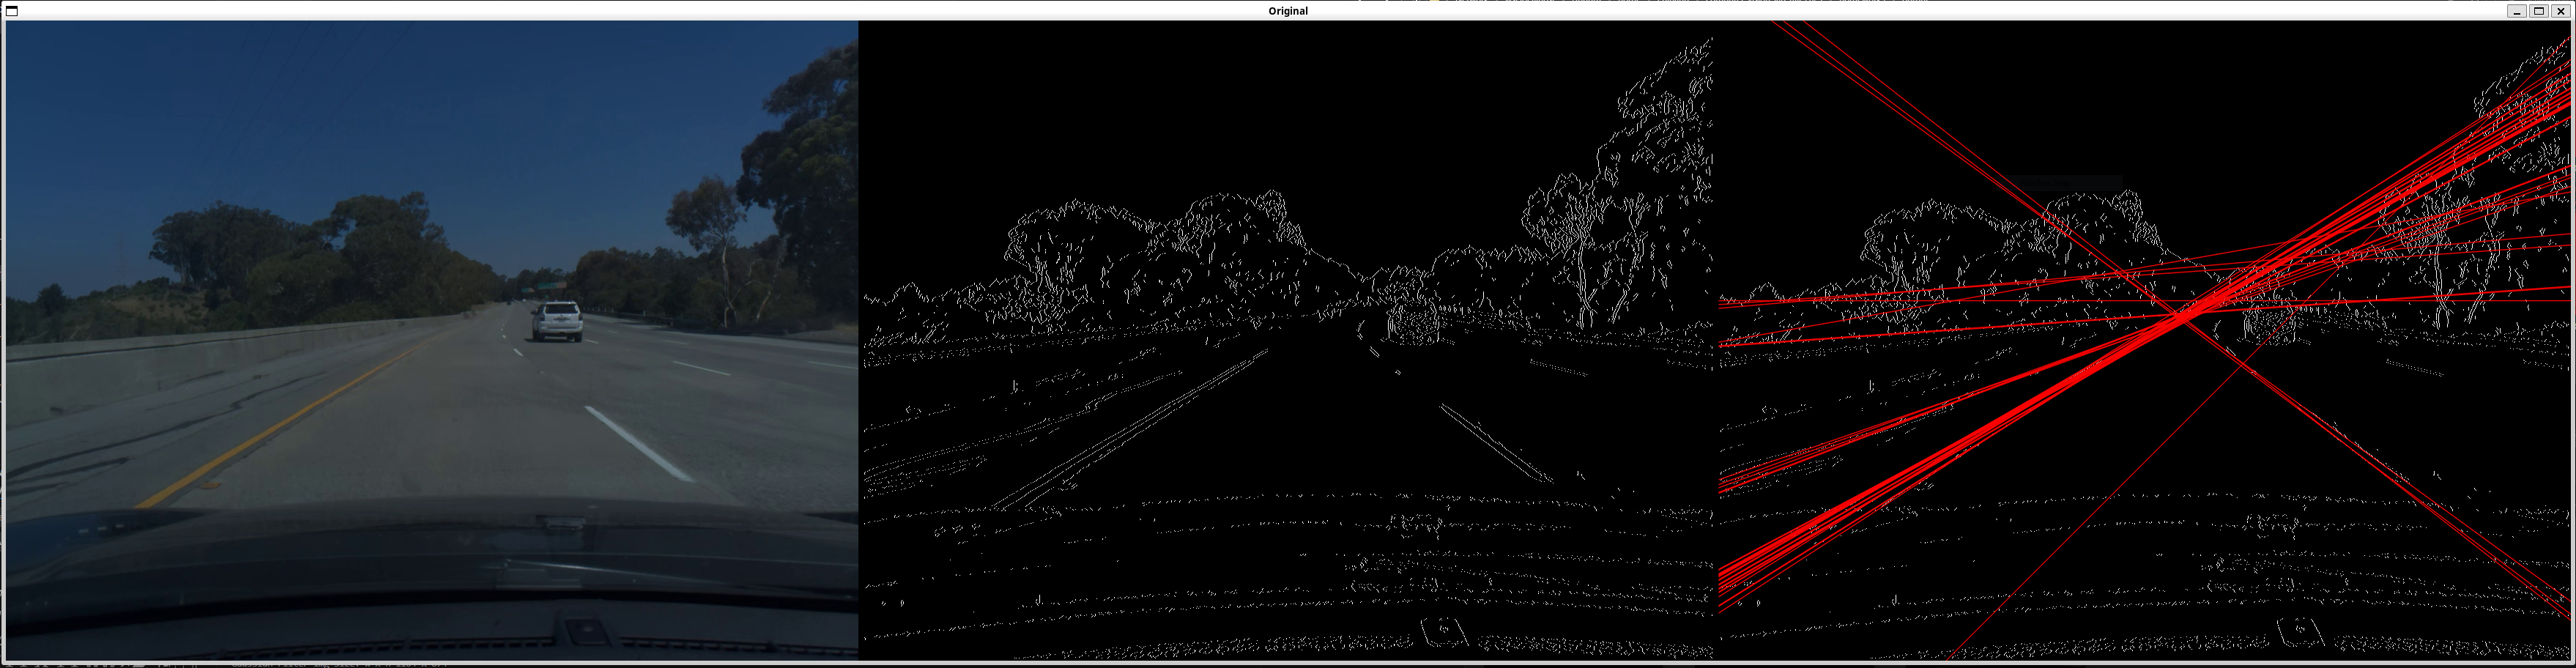
\includegraphics[width=1\linewidth]{program.png}
  \caption{Program Output (Automatic place image in frame)}
\end{figure}
\clearpage


\section{Applying Greyscale Filter}
\begin{tabular}{lll}
  Input  & : & Matrix of Input Image  \\
  Output & : & Matrix of Output Image \\
\end{tabular}
\begin{lstlisting}
Mat applyGreyscaleFilter(Mat img)
{
    // Create New Image as Output Image
    Mat bw_img(img.size(), img.type());
    for (int j = 0; j < img.rows; j++)
    {
        for (int i = 0; i < img.cols; i++)
        {
            // Get the pixel value from the original image
            Vec3b brg_px = img.at<Vec3b>(j, i);

            // Normal average function ie. sum(xn)/n ;
            int b = (brg_px[0] + brg_px[1] + brg_px[2]) / 3;

            // Write back to every channel
            brg_px[0] = b;
            brg_px[1] = b;
            brg_px[2] = b;

            // Write to new image buffer
            bw_img.at<Vec3b>(j, i) = brg_px;
        }
    }
    // return the output image
    return bw_img;
}
\end{lstlisting}
\begin{figure}[!htb]
  \centering
  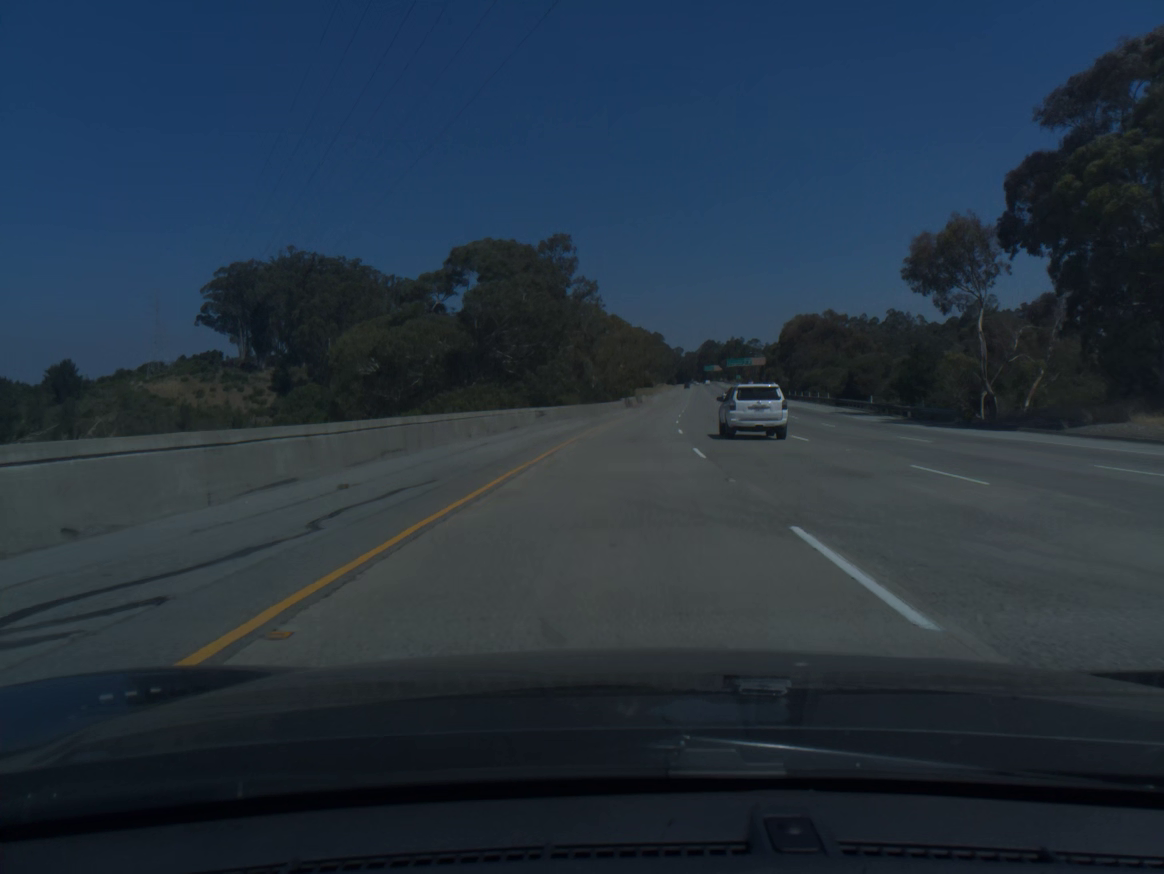
\includegraphics[height=0.4\paperheight]{test_img/img3.png}
  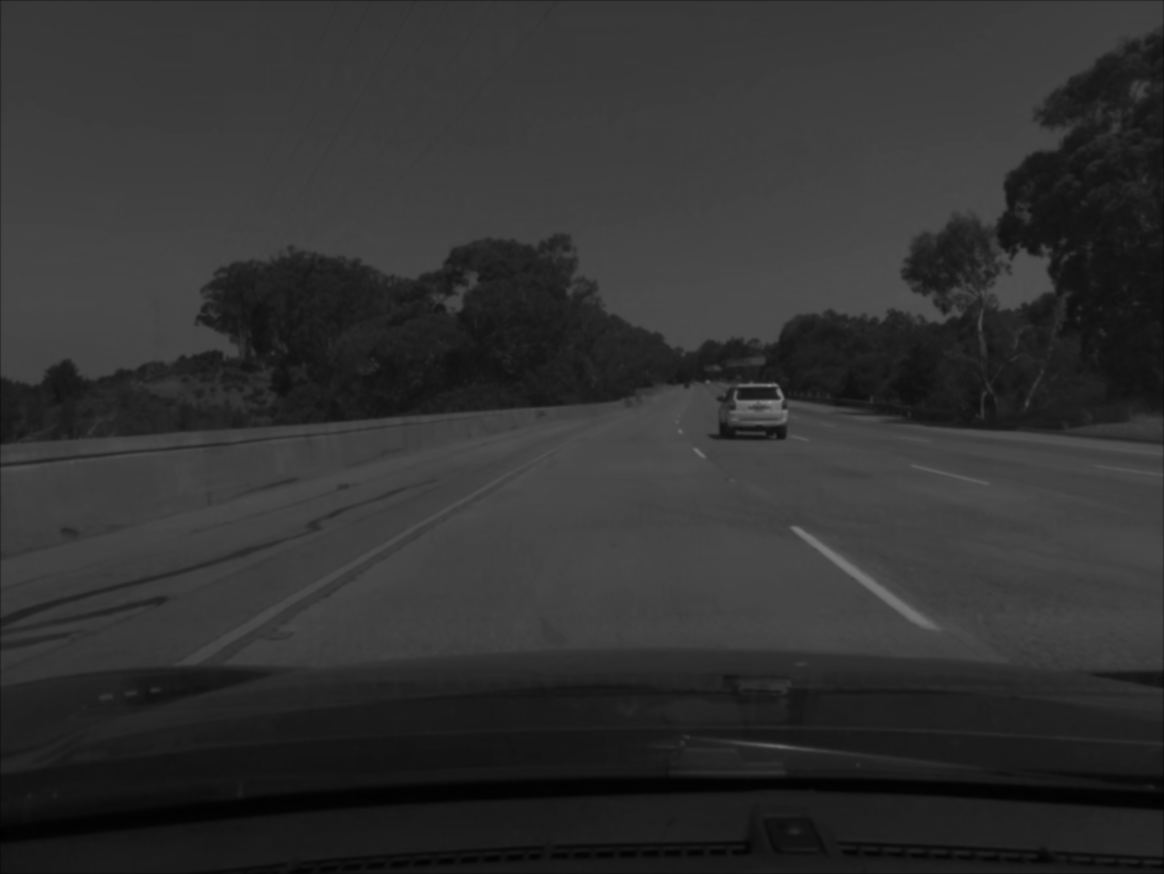
\includegraphics[height=0.4\paperheight]{result_img/img3_q1.png}
  \caption{Comparison Between (U) Original and (L) Mean Filter Applied Kernel=3, Padding=1}
\end{figure}
\clearpage

\section{Apply Gaussian Filter}
Since using filter can be reused in multiple step, the general function is extracted below.
In order to use Gaussian filter, we need to create kernel using provided function below, then applt with the general function.
\subsection{Create Gaussian Filter}
\begin{tabular}{lll}
  Input  & : & Kernel size (Integer)  \\
         &   & Sigma (float) \\
  Output & : & Matrix of Gaussian Filter \\
\end{tabular}
\begin{lstlisting}
float calculateGaussian(int x, int y, float sigma)
{
    return (1 / (CV_2PI * sigma * sigma)) * (powf32(K_E, -1 * ((x * x) + (y * y)) / (2 * sigma * sigma)));
}

Mat createGaussianFilter(int size, float sigma)
{
    int center = size / 2;
    Mat kernel = Mat::zeros(size, size, CV_32F);
    for (int j = 0; j < kernel.rows; j++)
    {
        for (int i = 0; i < kernel.cols; i++)
        {
            kernel.at<float>(j, i) = calculateGaussian(i - center, j - center, sigma);
        }
    }
    return kernel;
}
\end{lstlisting}

\subsection{Apply Filter}
\begin{tabular}{lll}
  Input  & : & Matrix of Input Image  \\
         &   & Kernel Matrix \\
         &   & Stride size (Integer)  \\
         &   & Suppress Border (Bool)  \\
  Output & : & Matrix of Output Image \\
\end{tabular}
\begin{lstlisting}
Mat applyFilter(Mat img, Mat kernel, int stride, bool suppress_border)
{

    // calculate kernel offset ie. number of pixel before and
    // after since the target pixel will be the center of
    // matrix,
    // in order to get the neighbour pixel with size of kernel
    // size, offset will be applied for both before, and after
    // the target pixel
    // example
    // width = 5 => offset = (int)5/2 = 2;
    // px   ... k   n-offset    ... n   ... n+offset    k
    int ker_x_offset = kernel.cols / 2;
    int ker_y_offset = kernel.rows / 2;

    int padding = ker_x_offset;

    // get kernel size
    int ker_w = kernel.cols;
    int ker_h = kernel.rows;

    // calculate output image size
    int out_w = ((img.cols + (2 * padding) - kernel.cols) / stride) + 1;
    int out_h = ((img.rows + (2 * padding) - kernel.rows) / stride) + 1;

    // create intermediate buffer and add padding, size is
    // w+(2*padding),h+(2*padding) then copy the content
    // of image to the buffer
    Mat padded;
    padded = Mat::zeros(img.rows + (2 * padding), img.cols + (2 * padding), CV_32SC3);
    int dtype = img.type();

    // here, we convert data type while copy to make it compatible
    // for higher precision computation
    // check if input is uint8 or int 32
    // if uint8 then we will channel-wise copy to padded buffer
    // due to different data alignment
    // if int38 then we will pixel-wise copy to padded buffer
    switch (dtype)
    {
    case CV_32SC3:
        for (int j = 0; j < img.rows; j++)
        {
            for (int i = 0; i < img.cols; i++)
            {
                padded.at<Vec3i>(j + padding, i + padding) = img.at<Vec3i>(j, i);
            }
        }
        break;
    case CV_8UC3:
        for (int j = 0; j < img.rows; j++)
        {
            for (int i = 0; i < img.cols; i++)
            {
                for (int k = 0; k < 3; k++)
                {
                    padded.at<Vec3i>(j + padding, i + padding)[k] = img.at<Vec3b>(j, i)[k];
                }
            }
        }
        break;
    default:
        break;
    }

    // create output buffer with calculated output size
    // data type need to be vector of signed int 32 bit
    // in case negative data is possible, this can help
    // preserve information through the convolution process
    // and rasterise to 8 bit at the last step
    Mat img_res = Mat::zeros(out_h, out_w, CV_32SC3);

    Vec3i res(0, 0, 0);

    // iterate over the size of input image
    for (int img_j = 0; img_j < img.rows; img_j += stride)
    {
        for (int img_i = 0; img_i < img.cols; img_i += stride)
        {
            // check if it is a border and suppress border if selected
            if (img_i < ker_w || img_j < ker_h || img_i > img.cols - ker_h - 1 || img_j > img.rows - ker_h - 1)
            {
                if (suppress_border)
                {
                    res = Vec3i(0, 0, 0);
                    img_res.at<Vec3i>((img_j) / stride, (img_i) / stride) = res;
                    continue;
                }
            }

            // get windowed matrix from the padded buffer with
            // the size of kernel size, and target pixel is in
            // the center of windowed matrix
            Mat windowed = padded(Rect(img_i, img_j, ker_w, ker_h));
            res = Vec3i(0, 0, 0);
            float tmp = 0;
            float tmp1 = 0;
            float tmp2 = 0;
            float tmp3 = 0;

            // item-wise multiply windowed matrix with kernel
            // matrix and summarise
            for (int ker_j = 0; ker_j < kernel.rows; ker_j++)
            {
                for (int ker_i = 0; ker_i < kernel.cols; ker_i++)
                {
                    Vec3b t = windowed.at<Vec3i>(ker_j, ker_i);
                    float k = kernel.at<float>(ker_j, ker_i);
                    tmp += (t[0] * k);
                    tmp1 += (t[0] * k);
                    tmp2 += (t[1] * k);
                    tmp3 += (t[2] * k);
                }
            }
            res[0] = tmp1;
            res[1] = tmp2;
            res[2] = tmp3;

            // write to output buffer
            img_res.at<Vec3i>((img_j) / stride, (img_i) / stride) = res;
        }
    }
    // return the output image
    return img_res;
}
\end{lstlisting}
\begin{figure}[!htb]
  \centering
  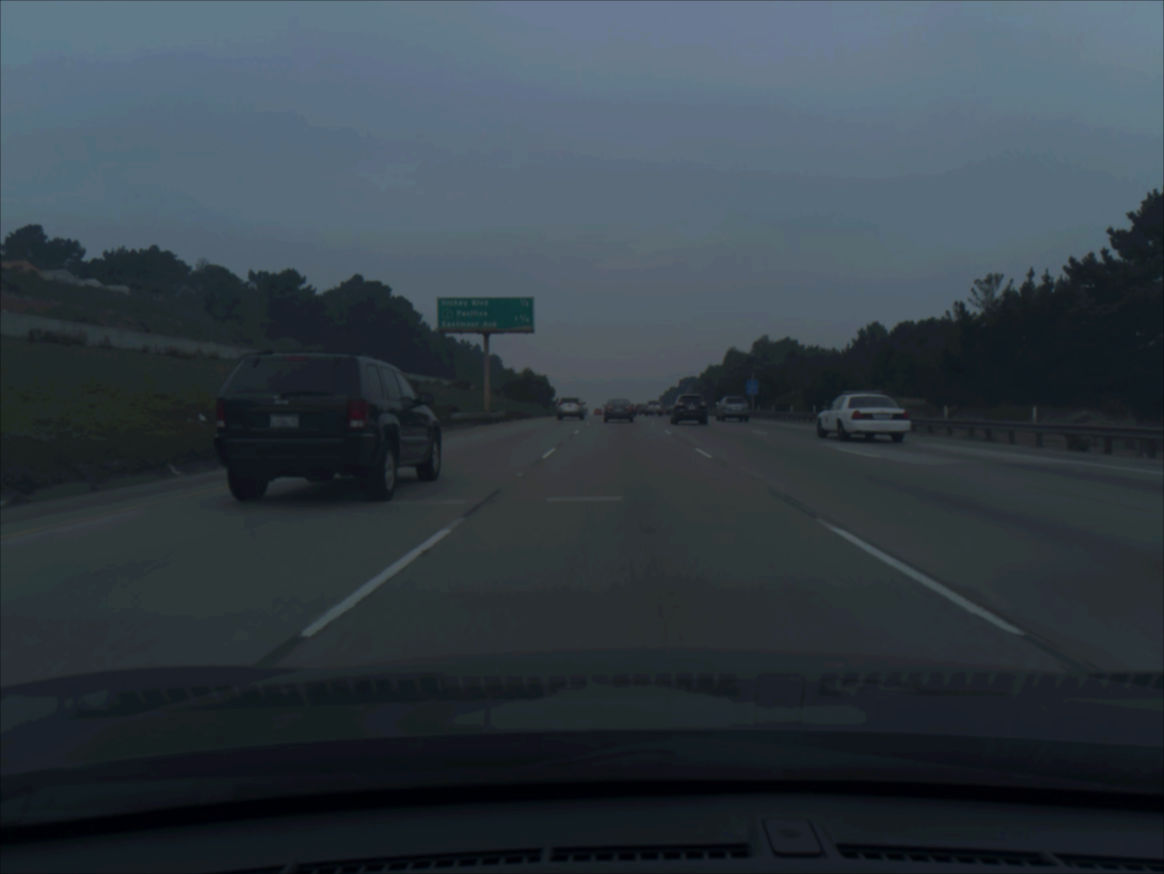
\includegraphics[height=0.4\paperheight]{output/img2_q1_K3_SIG_1.0.png}
  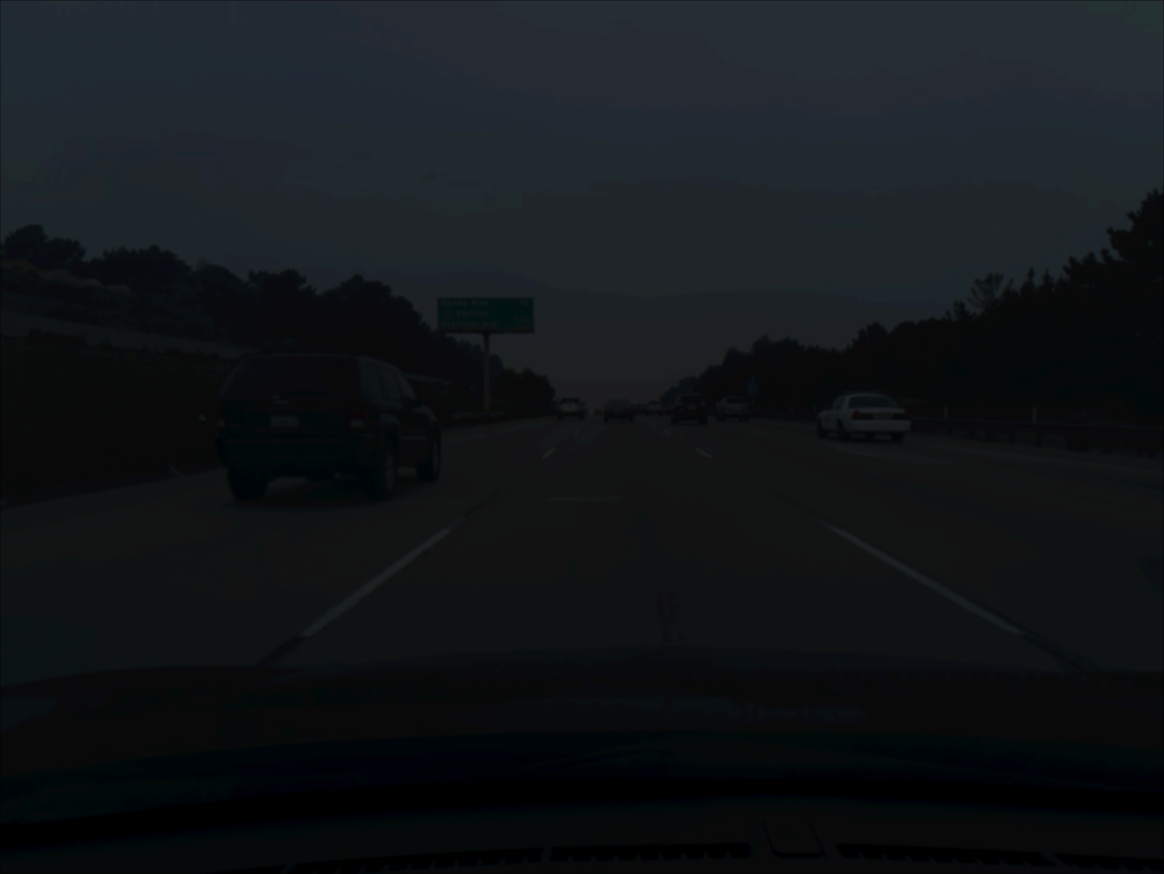
\includegraphics[height=0.4\paperheight]{output/img2_q1_K3_SIG_2.0.png}
  \caption{Comparison Between (U) Original and (L) Gaussian Filter Applied Kernel=3, Sigma=2}
\end{figure}
\clearpage


\section{Apply Canny Edge Detector}
In order to perform Canny Edge Detection, please follow step below
\subsection{Sobel X and Y}
This only apply Sobel kernel.
\begin{tabular}{lll}
  Input  & : & Matrix of Input Image  \\
  Output & : & Matrix of Output Image \\
\end{tabular}
\begin{lstlisting}
Mat applySobelX(Mat img_in)
{
    float c_sobelX[] = {-1, 0, 1,
                        -2, 0, 2,
                        -1, 0, 1};
    Mat sobelX(3, 3, CV_32F, c_sobelX);
    Mat result = applyFilter(img_in, sobelX, 1, true);
    return result;
}

Mat applySobelY(Mat img_in)
{
    float c_sobelY[] = {-1, -2, -1,
                          0,  0,  0,
                          1,  2,  1};
    Mat sobelY(3, 3, CV_32F, c_sobelY);
    Mat result = applyFilter(img_in, sobelY, 1, true);
    return result;
}
\end{lstlisting}
\begin{figure}[!htb]
  \centering
  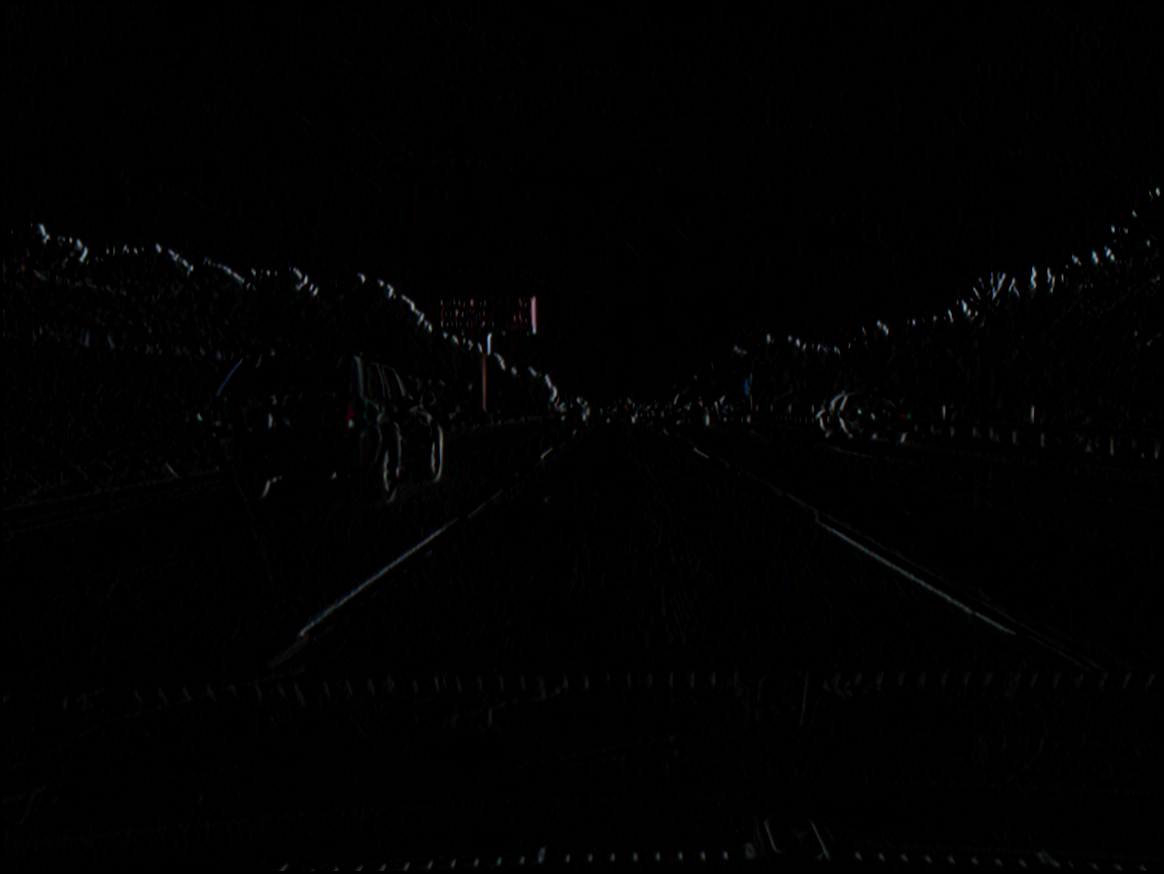
\includegraphics[height=0.4\paperheight]{output/img2_q2_SOBEL_X.png}
  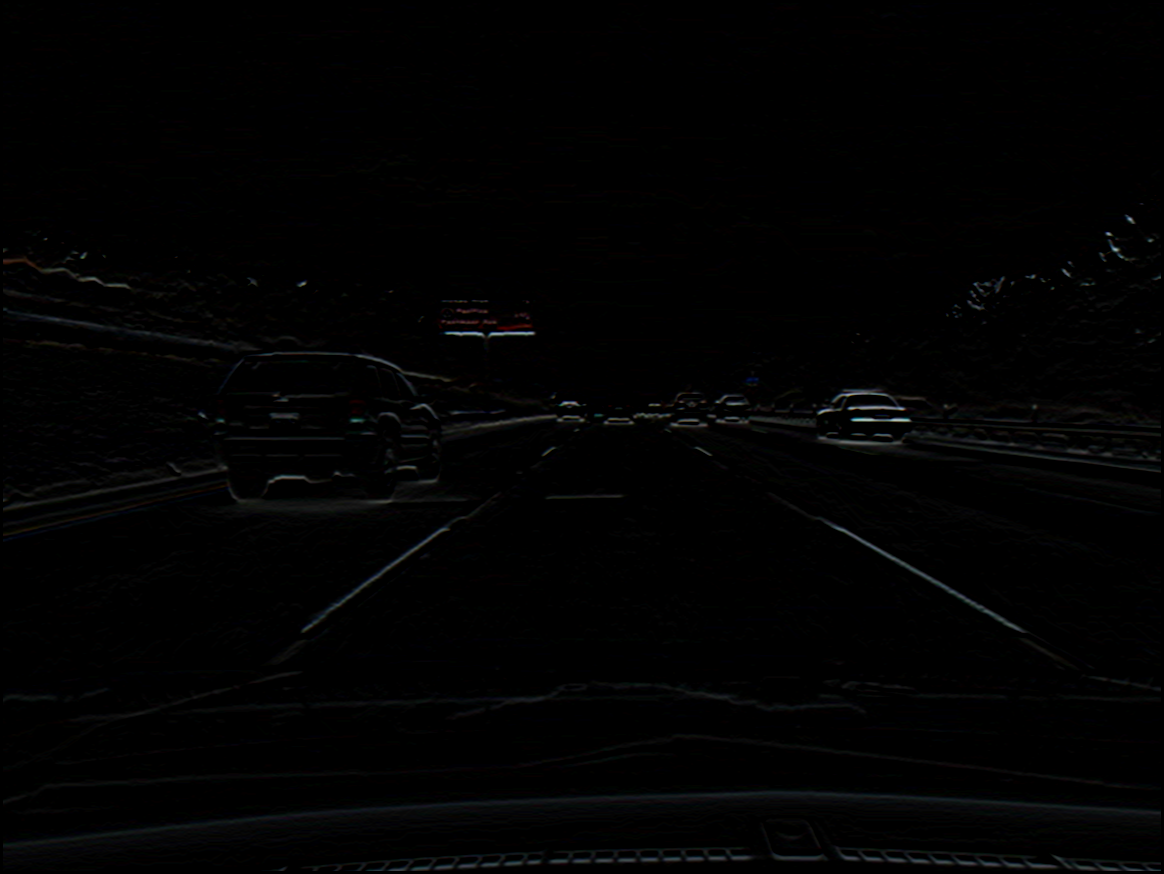
\includegraphics[height=0.4\paperheight]{output/img2_q2_SOBEL_Y.png}
  \caption{Comparison Between (U) Original and (L) Gaussian Filter Applied Kernel=3, Sigma=2}
\end{figure}
\clearpage


\subsection{Gradient Calculation}
This step, we will get edge strength and direction.

\subsubsection{Edge Strength}
\begin{tabular}{lll}
  Input  & : & Matrix of Input Sobel X  \\
         & : & Matrix of Input Sobel Y  \\
  Output & : & Matrix of Edge Strength \\
\end{tabular}
\begin{lstlisting}
Mat calculateEdgeStrength(Mat x, Mat y)
{
    Mat strength = Mat::zeros(x.rows, x.cols, CV_32FC3);
    float tmp = 0;
    for (int j = 0; j < strength.rows; j += 1)
    {
        for (int i = 0; i < strength.cols; i += 1)
        {
            for (int k = 0; k < 3; k++)
            {
                // Strength of pixel is calculated by
                // sqrt(gx^2 + gy^2)
                tmp = (x.at<Vec3i>(j, i)[k] * x.at<Vec3i>(j, i)[k]) + (y.at<Vec3i>(j, i)[k] * y.at<Vec3i>(j, i)[k]);
                strength.at<Vec3f>(j, i)[k] = sqrtf32(tmp);
            }
        }
    }

    return strength;
}
\end{lstlisting}
\begin{figure}[!htb]
  \centering
  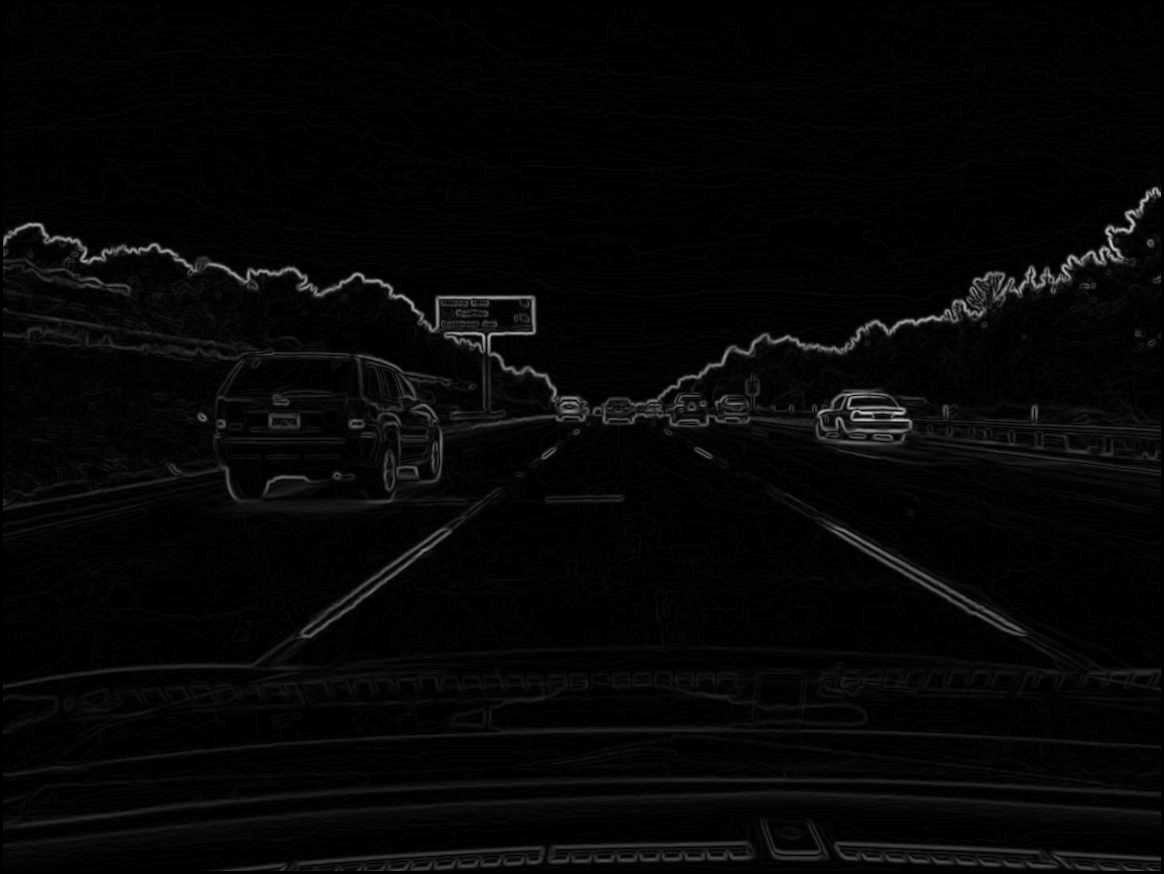
\includegraphics[height=0.4\paperheight]{output/img2_q2_EDGE_STRENGTH.png}
  \caption{Edge Strength}
\end{figure}
\clearpage

\subsubsection{Edge Direction}
\begin{tabular}{lll}
  Input  & : & Matrix of Input Sobel X  \\
         & : & Matrix of Input Sobel Y  \\
  Output & : & Matrix of Edge Direction \\
\end{tabular}
\begin{lstlisting}
Mat calculateEdgeDirection(Mat x, Mat y)
{
    Mat direction = Mat::zeros(x.rows, x.cols, CV_32FC3);
    for (int j = 0; j < direction.rows; j += 1)
    {
        for (int i = 0; i < direction.cols; i += 1)
        {
            for (int k = 0; k < 3; k++)
            {
                // direction of pixel is calculated by
                // atan(y/x)
                direction.at<Vec3f>(j, i)[k] = atan2f32(y.at<Vec3f>(j, i)[k], x.at<Vec3f>(j, i)[k]) * 10;
            }
        }
    }
    return direction;
}
\end{lstlisting}
\begin{figure}[!htb]
  \centering
  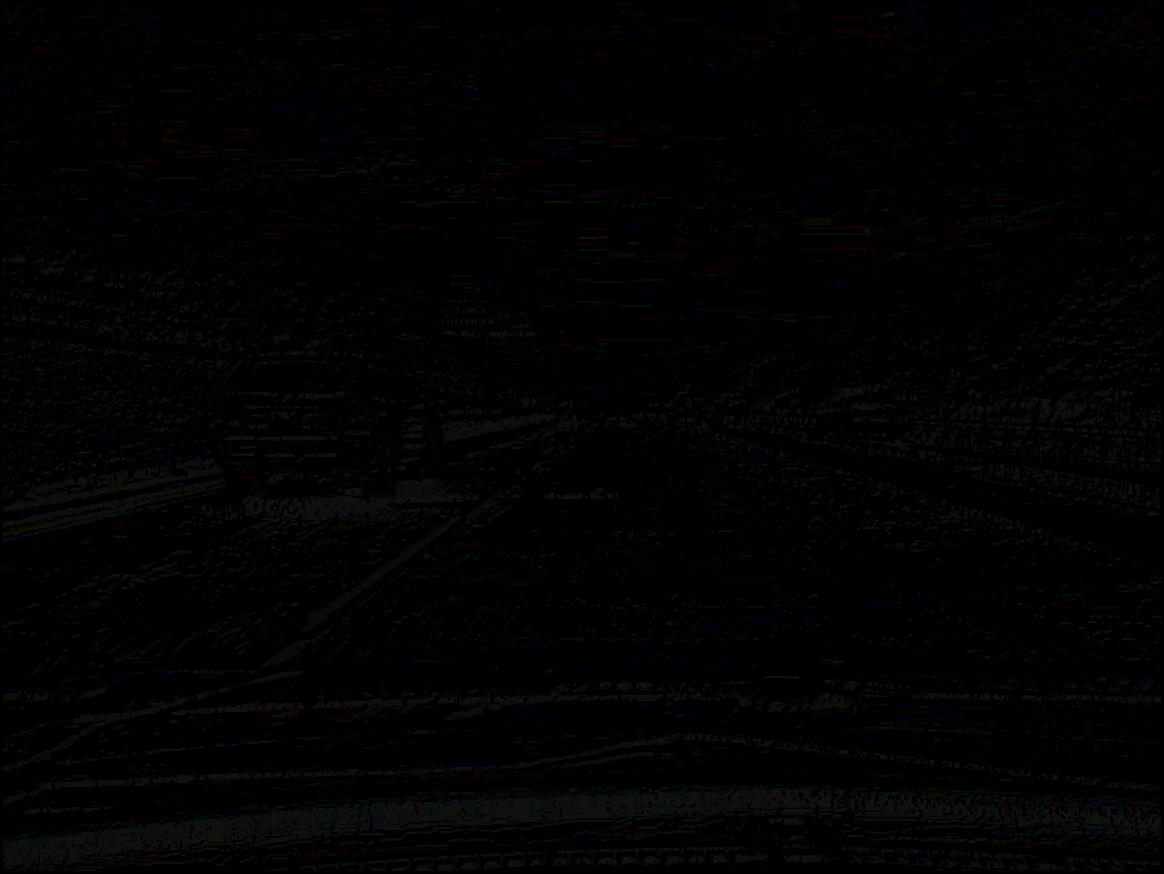
\includegraphics[height=0.4\paperheight]{output/img2_q2_EDGE_DIR.png}
  \caption{Direction of Gradient}
\end{figure}
\clearpage

\subsection{Non Maximum Suppression}
This function will thinner the edge.
\begin{tabular}{lll}
  Input  & : & Matrix of Input Edge Strength  \\
         & : & Matrix of Input Edge Direction  \\
  Output & : & Matrix of NMS Image \\
\end{tabular}
\begin{lstlisting}
int quantiseDirection(float angle)
{
    // convert radiant to degree
    angle = angle * 180 / CV_PI;

    // quantise to 4 axes 
    if ((angle >= 0 && angle < 22.5) || (angle >= 157.5 && angle <= 180))
    {
        return 0;
    }
    else if (angle >= 22.5 && angle < 67.5)
    {
        return 45;
    }
    else if (angle >= 67.5 && angle < 112.5)
    {
        return 90;
    }
    else if (angle >= 112.5 && angle < 157.5)
    {
        return 135;
    }
    else
    {
        return 0;
    }
}

Mat calculateNonMaximumSuppression(cv::Mat strength, cv::Mat direction)
{
    // Create a zero-initialized matrix with the same size as the input, to store the result
    Mat res = Mat::zeros(strength.rows, strength.cols, CV_32SC3);

    // Iterate over the image, avoiding the borders (as the algorithm needs neighboring pixels)
    for (int j = 1; j < strength.rows - 1; j++)
    {
        for (int i = 1; i < strength.cols - 1; i++)
        {
            // Iterate over each channel (assuming a 3-channel image)
            for (int k = 0; k < 3; k++)
            {
                // Quantize the direction to one of the four possible angles (0, 45, 90, 135)
                int dir = quantiseDirection(direction.at<Vec3f>(j, i)[k]);

                // Retrieve the strength of the neighboring pixels in all 8 directions
                float neighbour_UL = strength.at<Vec3f>(j - 1, i - 1)[k];
                float neighbour_UM = strength.at<Vec3f>(j - 1, i)[k];
                float neighbour_UR = strength.at<Vec3f>(j - 1, i + 1)[k];
                float neighbour_ML = strength.at<Vec3f>(j, i - 1)[k];
                float neighbour_CC = strength.at<Vec3f>(j, i)[k]; // Current pixel
                float neighbour_MR = strength.at<Vec3f>(j, i + 1)[k];
                float neighbour_DL = strength.at<Vec3f>(j + 1, i - 1)[k];
                float neighbour_DM = strength.at<Vec3f>(j + 1, i)[k];
                float neighbour_DR = strength.at<Vec3f>(j + 1, i + 1)[k];

                // Initially set the result pixel to the current strength
                res.at<Vec3i>(j, i)[k] = (int)neighbour_CC;

                // Depending on the quantized direction, suppress non-maximum pixels
                // by setting them to zero if they are not the local maxima along the gradient direction
                switch (dir)
                {
                case 0:
                    if (neighbour_CC <= neighbour_ML || neighbour_CC <= neighbour_MR)
                        res.at<Vec3f>(j, i)[k] = 0;
                    break;
                case 45:
                    if (neighbour_CC <= neighbour_UR || neighbour_CC <= neighbour_DL)
                        res.at<Vec3f>(j, i)[k] = 0;
                    break;
                case 90:
                    if (neighbour_CC <= neighbour_UM || neighbour_CC <= neighbour_DM)
                        res.at<Vec3f>(j, i)[k] = 0;
                    break;
                case 135:
                    if (neighbour_CC <= neighbour_UL || neighbour_CC <= neighbour_DR)
                        res.at<Vec3f>(j, i)[k] = 0;
                    break;
                }
            }
        }
    }

    // Return the resulting image after non-maximum suppression
    return res;
}
\end{lstlisting}
\begin{figure}[!htb]
  \centering
  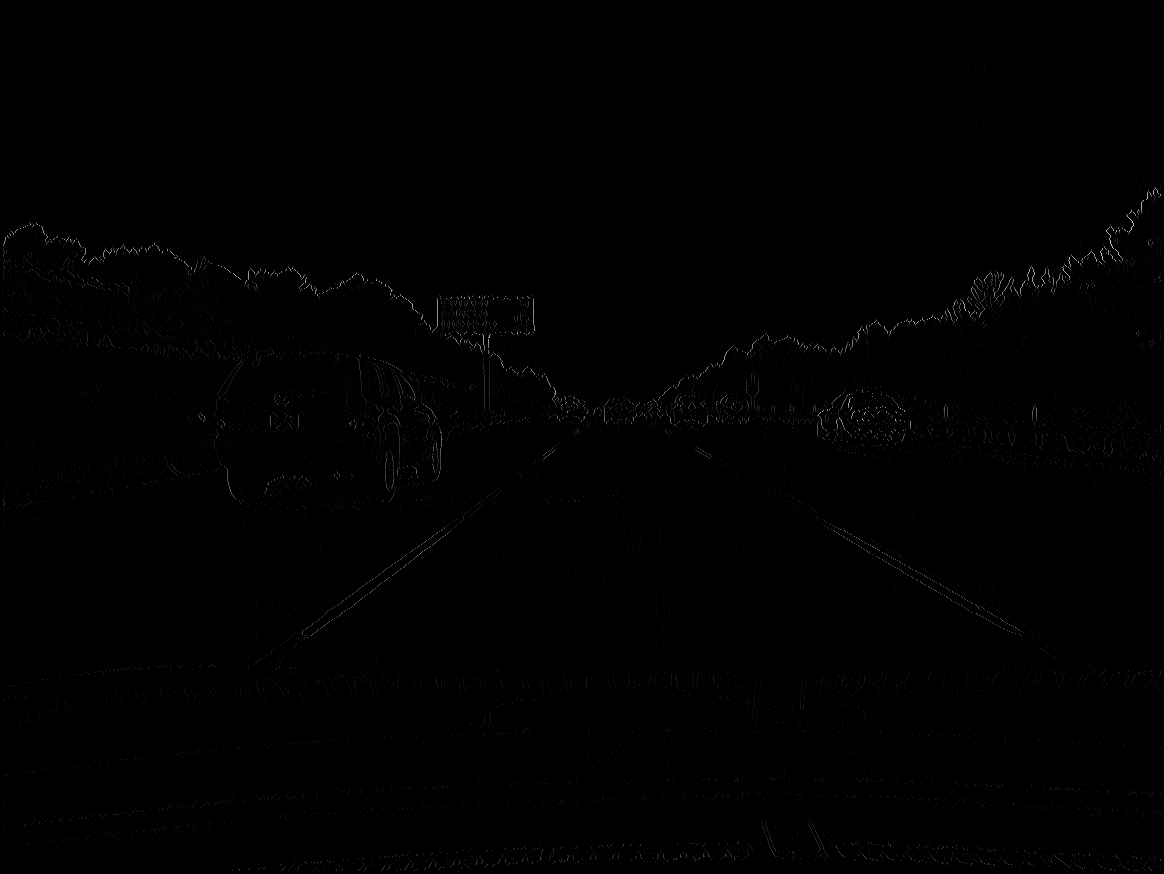
\includegraphics[height=0.4\paperheight]{output/img2_q2_NMS.png}
  \caption{Thinned Edge Image}
\end{figure}
\clearpage

\subsection{Double Thresholding}
\begin{tabular}{lll}
  Input  & : & Matrix of Input NMS  \\
         & : & Low Threshold (Integer)  \\
         & : & High Threshold (Integer)  \\
  Output & : & Matrix of Output Image \\
\end{tabular}
\begin{lstlisting}
Mat applyDoubleThresholding(Mat input, int thres_low, int thres_high)
{
    // Create a zero-initialized matrix with the same size as the input, to store the result
    Mat res = Mat::zeros(input.rows, input.cols, CV_8UC3);

    // Temporary variable to store the intensity of the current pixel
    int tmp = 0;

    // Iterate over the image, avoiding the borders
    for (int j = 1; j < input.rows - 1; j++)
    {
        for (int i = 1; i < input.cols - 1; i++)
        {
            // Iterate over each channel of the pixel
            for (int k = 0; k < 3; k++)
            {
                // Get the intensity value of the current pixel
                tmp = input.at<Vec3i>(j, i)[k];

                // If the intensity is higher than the high threshold, mark it as a strong edge (255)
                if (tmp >= thres_high)
                {
                    res.at<Vec3b>(j, i)[k] = 255;
                }
                // If the intensity is lower than the low threshold, suppress it (0)
                else if (tmp < thres_low)
                {
                    res.at<Vec3b>(j, i)[k] = 0;
                }
                // If the intensity is between the low and high thresholds, mark it as a weak edge (128)
                else
                {
                    res.at<Vec3b>(j, i)[k] = 128;
                }
            }
        }
    }

    // Return the resulting image after double thresholding
    return res;
}
\end{lstlisting}
\begin{figure}[!htb]
  \centering
  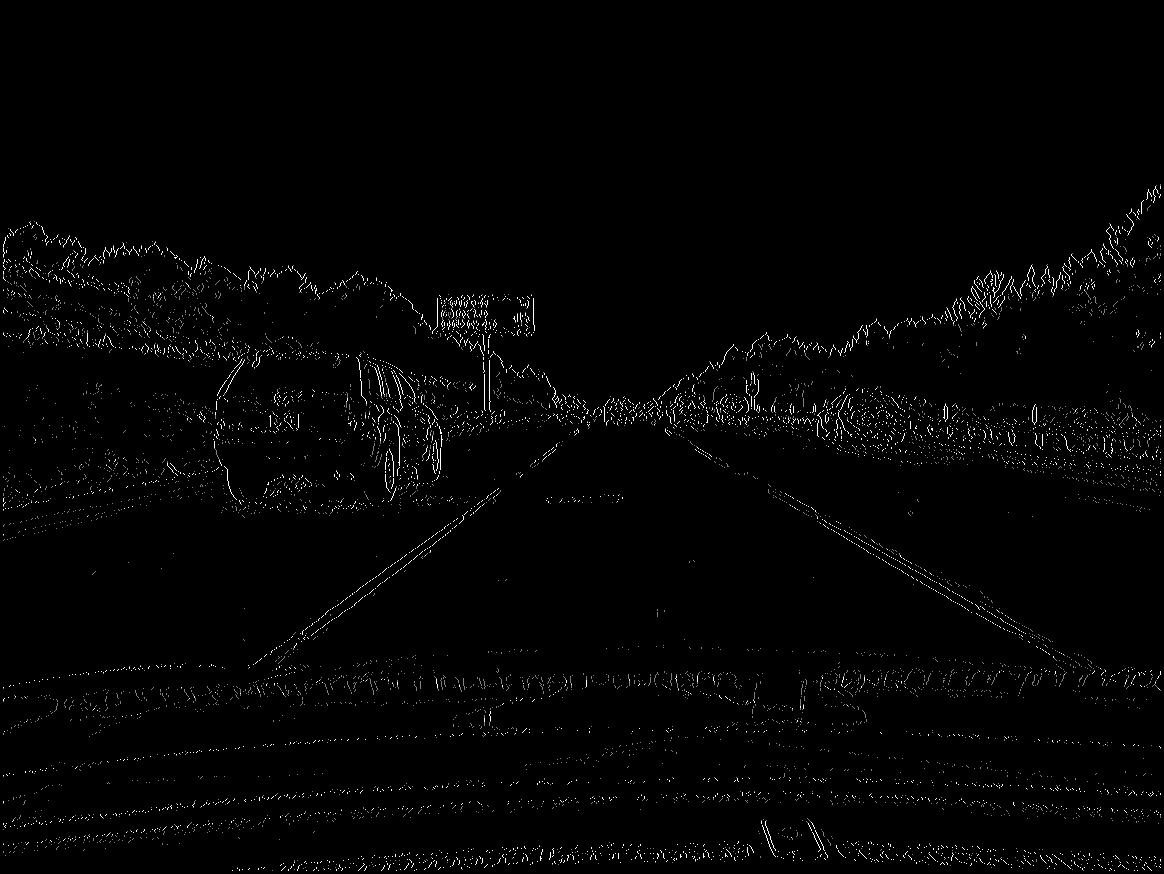
\includegraphics[height=0.4\paperheight]{output/img2_q2_DTS.png}
  \caption{Soft and Hard Edge Image}
\end{figure}
\clearpage

\subsection{Hysteresis Edge Tracking}
\begin{tabular}{lll}
  Input  & : & Matrix of Input Hard and Soft Edge Image  \\
  Output & : & Matrix of Output Image \\
\end{tabular}
\begin{lstlisting}
Mat applyHysteresis(Mat input)
{
    // Clone the input image to preserve the original and work on a copy
    Mat res = input.clone();

    // Define constants for weak and strong edge values
    int WEAK = 128, STRONG = 255;

    // Iterate over the image, avoiding the borders
    for (int j = 1; j < res.rows - 1; j++)
    {
        for (int i = 1; i < res.cols - 1; i++)
        {
            // Iterate over each channel of the pixel
            for (int k = 0; k < 3; k++)
            {
                // Check if the current pixel is a weak edge
                if (res.at<Vec3b>(j, i)[k] == WEAK)
                {
                    // Initialize a flag to check if the weak edge is connected to a strong edge
                    bool connected = false;

                    // Check the 8 neighboring pixels to see if any of them is a strong edge
                    for (int dj = -1; dj <= 1; ++dj)
                    {
                        for (int di = -1; di <= 1; ++di)
                        {
                            // Skip the current pixel
                            if (di == 0 && dj == 0)
                                continue;

                            // If a strong edge is found in the neighborhood, set the flag
                            if (res.at<Vec3b>(j + dj, i + di)[k] == STRONG)
                            {
                                connected = true;
                                break;
                            }
                        }
                        if (connected)
                            break;
                    }

                    // If the weak edge is connected to a strong edge, strengthen it; otherwise, suppress it
                    res.at<Vec3b>(j, i)[k] = connected ? STRONG : 0;
                }
            }
        }
    }

    // Return the resulting image after applying hysteresis
    return res;
}
\end{lstlisting}
\begin{figure}[!htb]
  \centering
  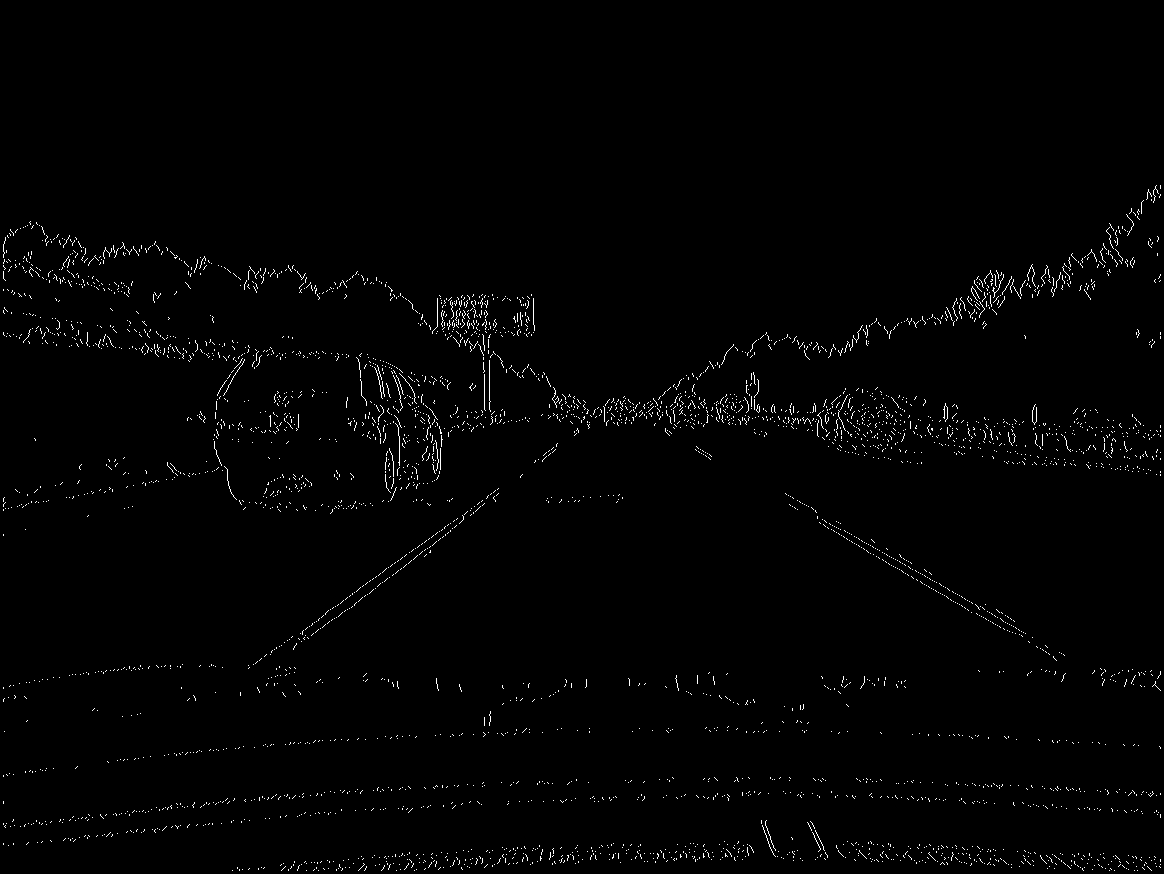
\includegraphics[height=0.4\paperheight]{output/img2_q2_HYS.png}
  \caption{Hard Edge Image}
\end{figure}
\clearpage

\section{Hough Transform}
After get the line, we need to add to image later
\begin{tabular}{lll}
  Input  & : & Matrix of Input Edge Strength  \\
         & : & List to store line (Vector) \\
         & : & Rho step (Float)\\
         & : & Theta step (Float) \\
         & : & Threshold (Integer)\\
\end{tabular}
\begin{lstlisting}
void applyHoughTransform(cv::Mat edges, std::vector<cv::Vec2f> &lines, float rho, float theta, int threshold)
{
    // Get the dimensions of the edges image
    int width = edges.cols;
    int height = edges.rows;

    // Calculate the maximum distance (rho) possible in the image
    int rho_max = (int)(std::sqrt(width * width + height * height));

    // Calculate the maximum number of bins for theta
    int theta_max = (int)(CV_PI / theta);

    // Create the accumulator matrix initialized to zero
    cv::Mat accum = cv::Mat::zeros(2 * rho_max, theta_max, CV_32S);

    // Iterate over the pixels of the edges image
    for (int y = 0; y < edges.rows; y++)
    {
        for (int x = 0; x < edges.cols; x++)
        {
            // Check if the current pixel is part of an edge
            if (edges.at<Vec3b>(y, x)[0] > 0)
            {
                // For each angle theta, calculate the corresponding rho value
                for (int t = 0; t < theta_max; t++)
                {
                    double current_theta = (t * theta);

                    // Calculate rho for the current (x, y) point and theta
                    double rho_val = cvRound((x * std::cos(current_theta)) + (y * std::sin(current_theta)));
                    int rho_index = (int)((rho_val / rho) + rho_max);

                    // Increment the accumulator's bin if the index is valid
                    if (rho_index >= 0 && rho_index < 2 * rho_max)
                    {
                        accum.at<int>(rho_index, t)++;
                    }
                }
            }
        }
    }

    // Iterate over the accumulator to find local maxima (lines)
    for (int r = 0; r < 2 * rho_max; r++)
    {
        for (int t = 0; t < theta_max; t++)
        {
            // If the bin's value is above the threshold, it is considered a line
            if (accum.at<int>(r, t) >= threshold)
            {
                // Convert (rho, theta) from accumulator space to image space and add to the lines vector
                lines.push_back(cv::Vec2f(r * rho - rho_max, t * theta));
            }
        }
    }
}  
\end{lstlisting}
\begin{figure}[!htb]
  \centering
  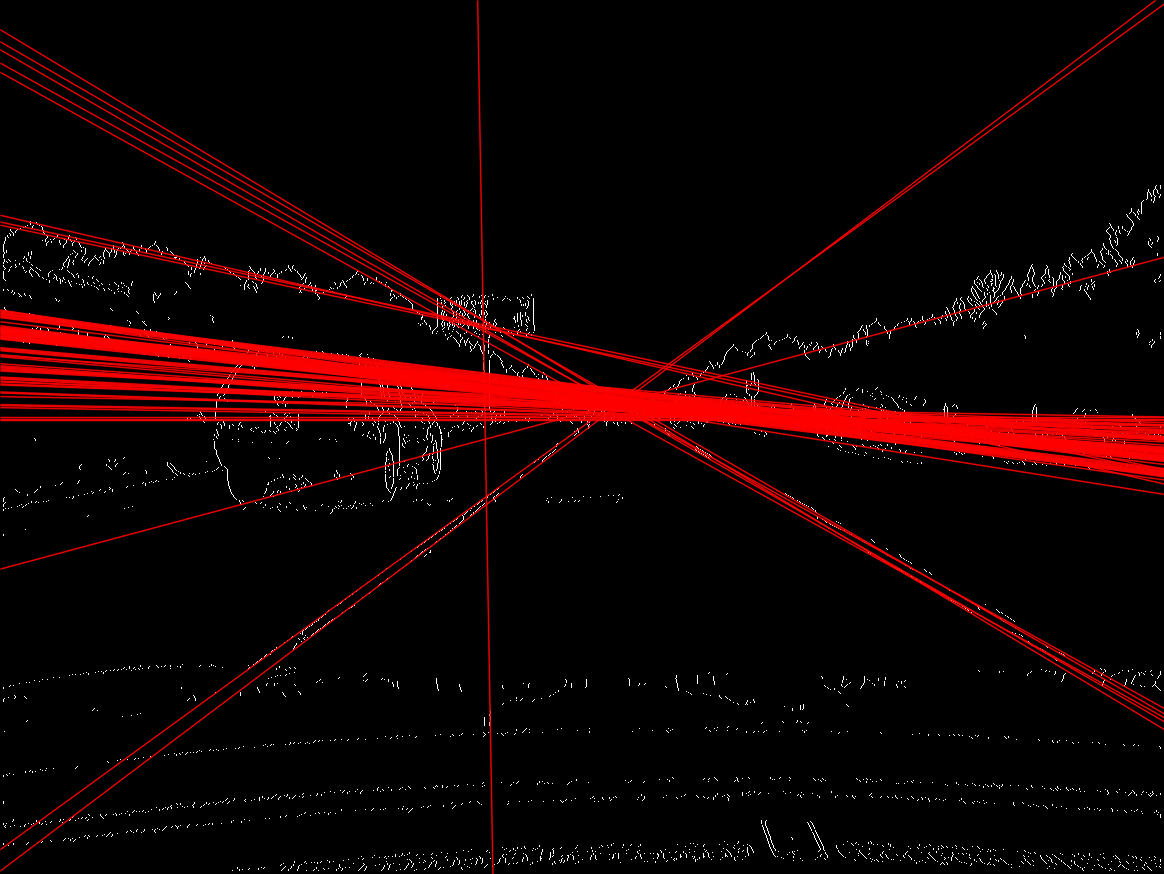
\includegraphics[height=0.4\paperheight]{result_img/img2_q3.png}
  \caption{Hough Transform Image}
\end{figure}
\clearpage



\chapter{Discussion}
\section{Observations}
\subsection{Parameters in Gaussian Filter}
\paragraph*{}
Sigma affects the output directly. Lower sigma tends to give more weight to the center of kernel. On the other hand, Higher distributes weight more. Kernel size also affect the output depends on sigma. For instance, using K=3 and sigma=1.0, the sum of weight is only 0.73, which is affect the result brightness as shown below. Higher sigma with small kernel will give darker image.
\begin{figure}[!htb]
  \begin{minipage}{\linewidth}
    \centering
    \begin{subfigure}{0.49\textwidth}
      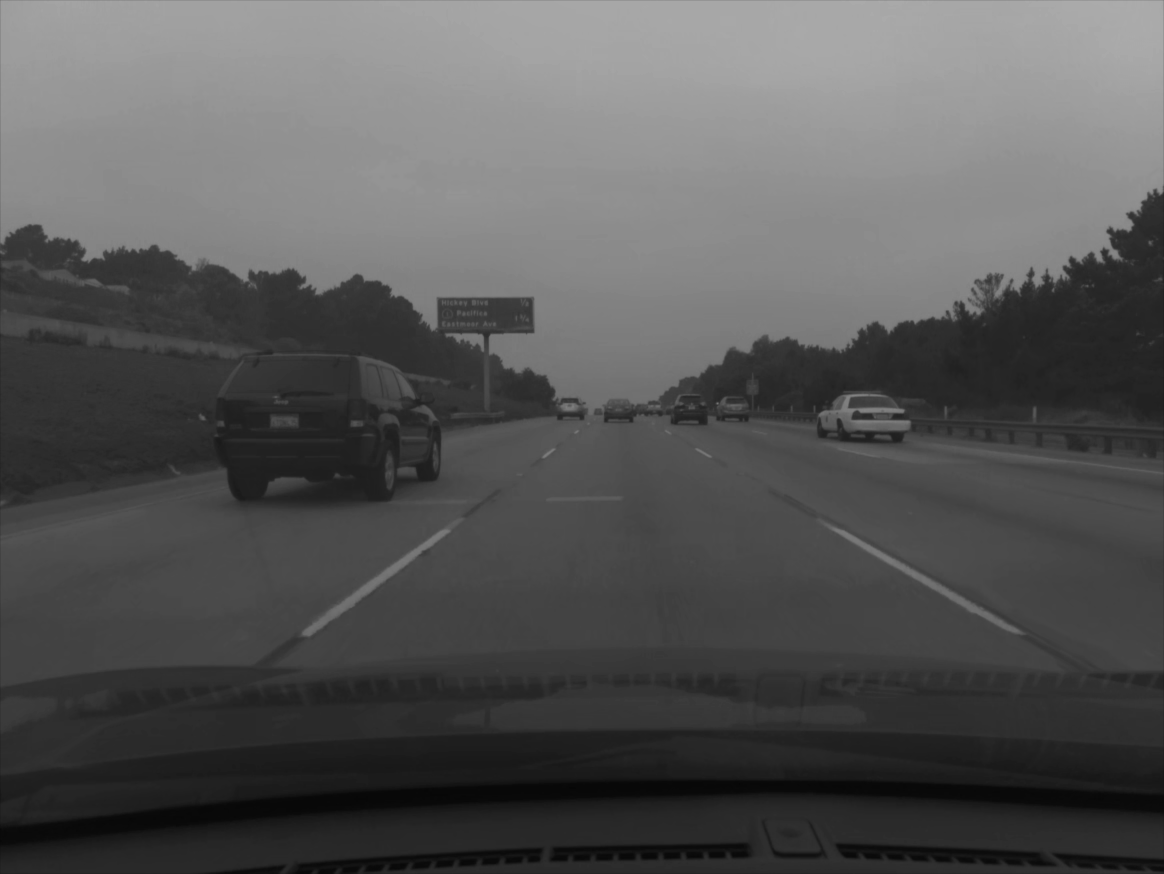
\includegraphics[width=\linewidth]{output/img2_q1_K3_SIG_0.5.png}
      \subcaption{sigma=0.5}
    \end{subfigure}
    \begin{subfigure}{0.49\textwidth}
      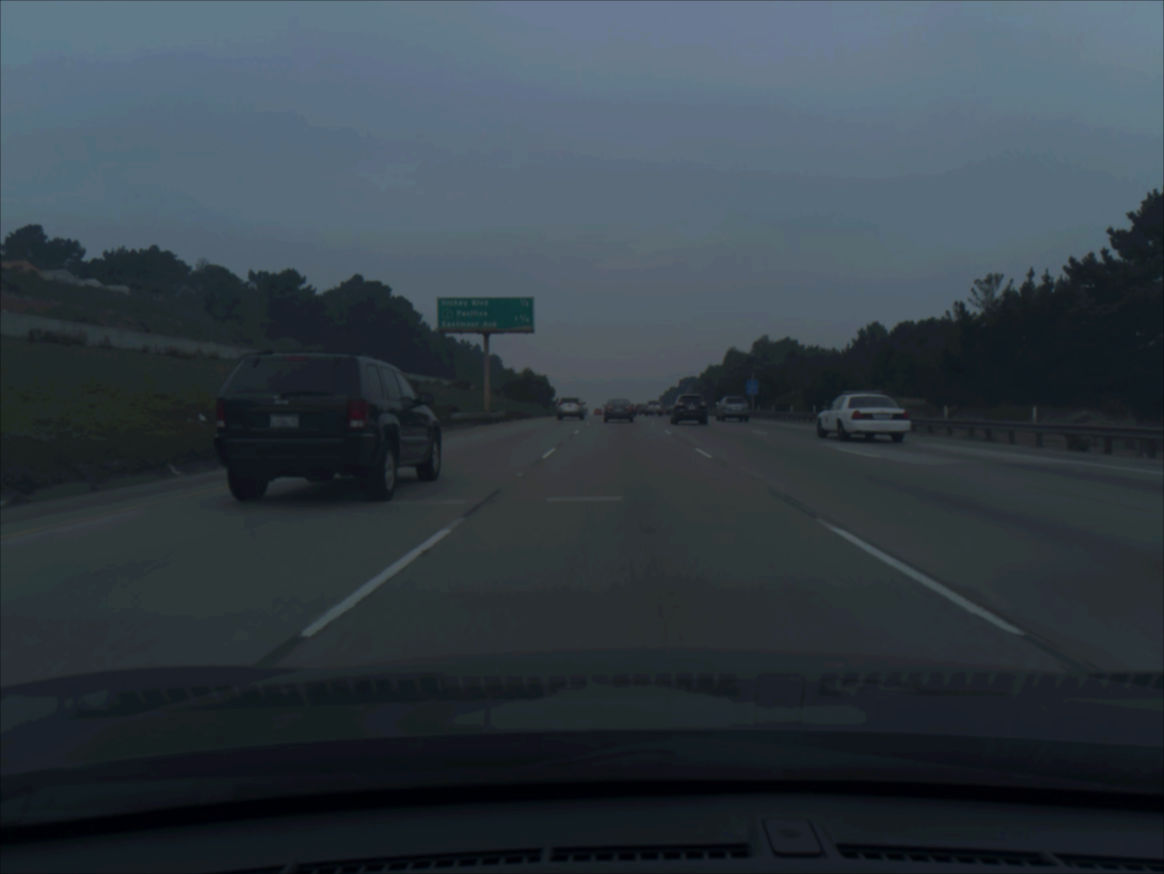
\includegraphics[width=\linewidth]{output/img2_q1_K3_SIG_1.0.png}
      \subcaption{sigma=1}
    \end{subfigure}
    

    \begin{subfigure}{0.49\textwidth}
      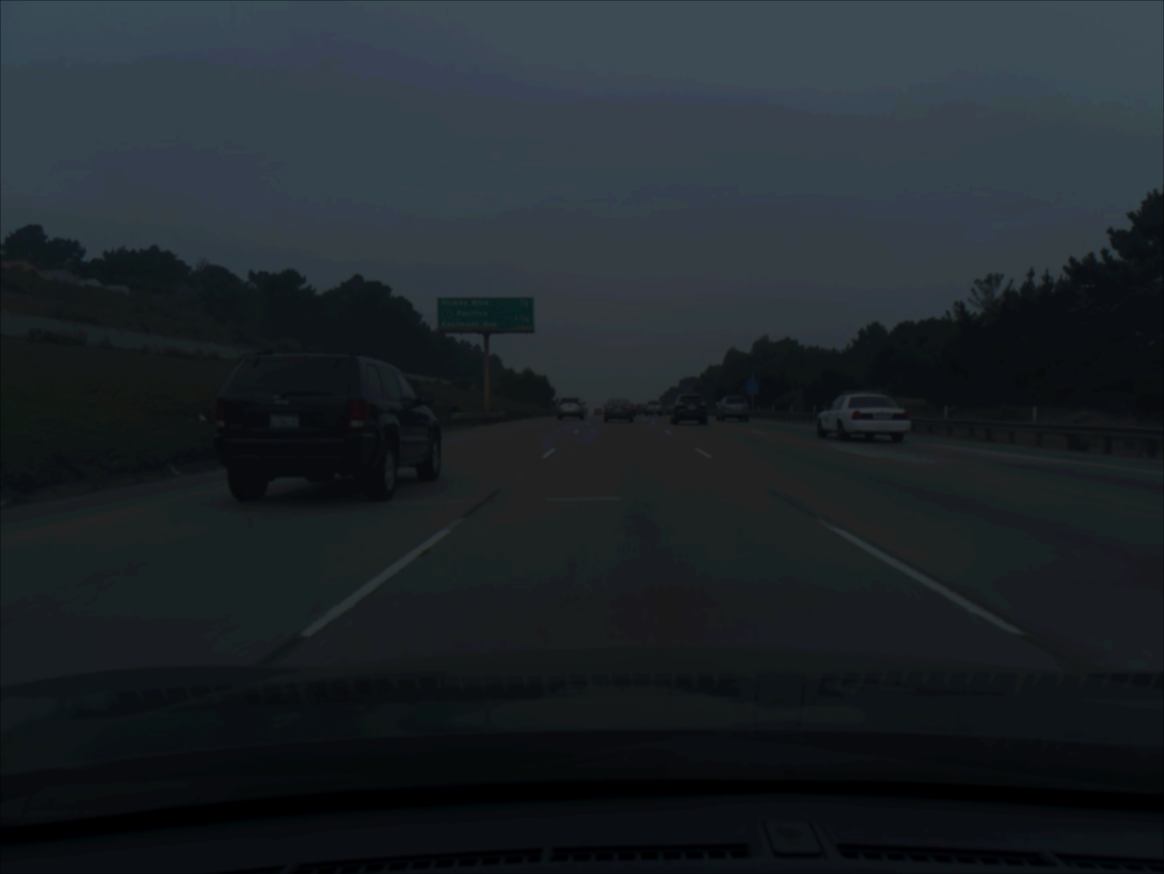
\includegraphics[width=\linewidth]{output/img2_q1_K3_SIG_1.5.png}
      \subcaption{sigma=1.5}
    \end{subfigure}
    \begin{subfigure}{0.49\textwidth}
      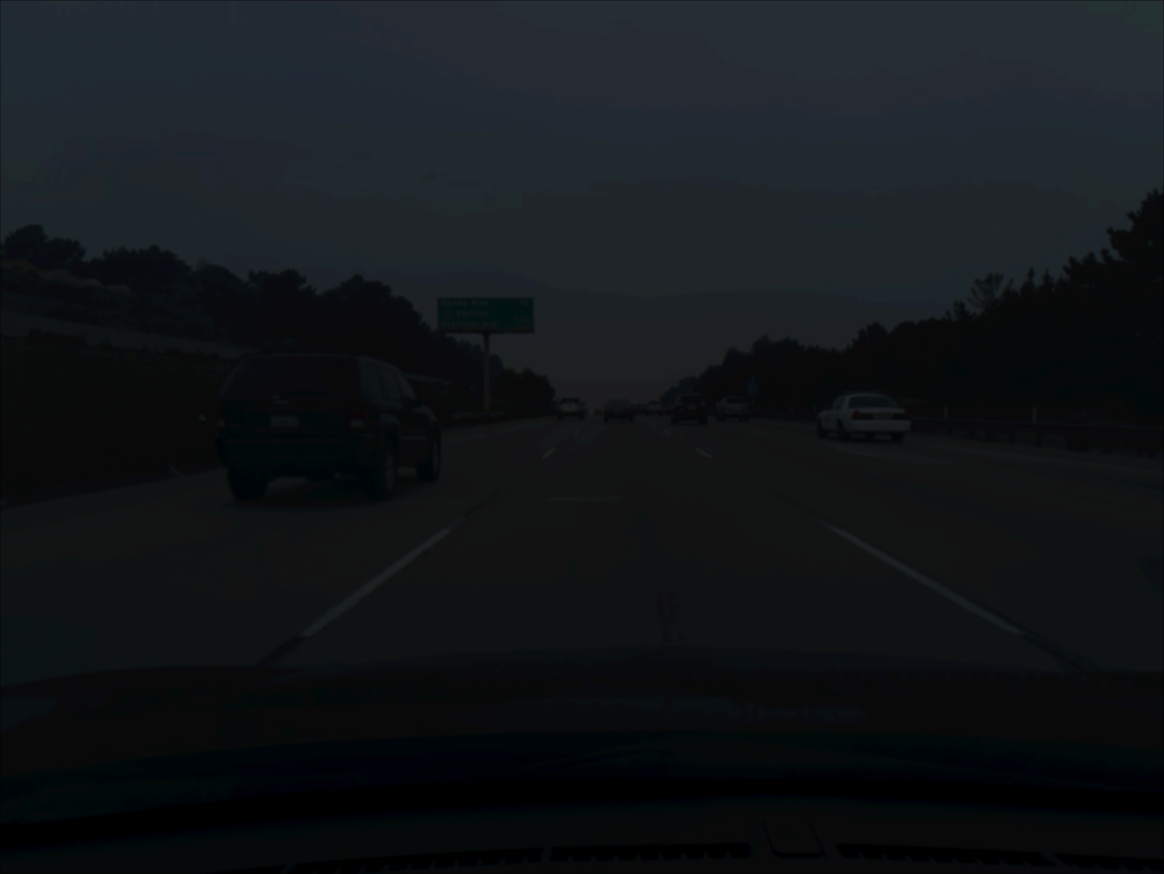
\includegraphics[width=\linewidth]{output/img2_q1_K3_SIG_2.0.png}
      \subcaption{sigma=2}
    \end{subfigure}

    \caption{Comparison of sigma on output brightness}
  \end{minipage}

\end{figure}


% \begin{figure}[!htb]
%   \begin{minipage}{\linewidth}
%     \centering
%     \begin{subfigure}{1\textwidth}
%       % 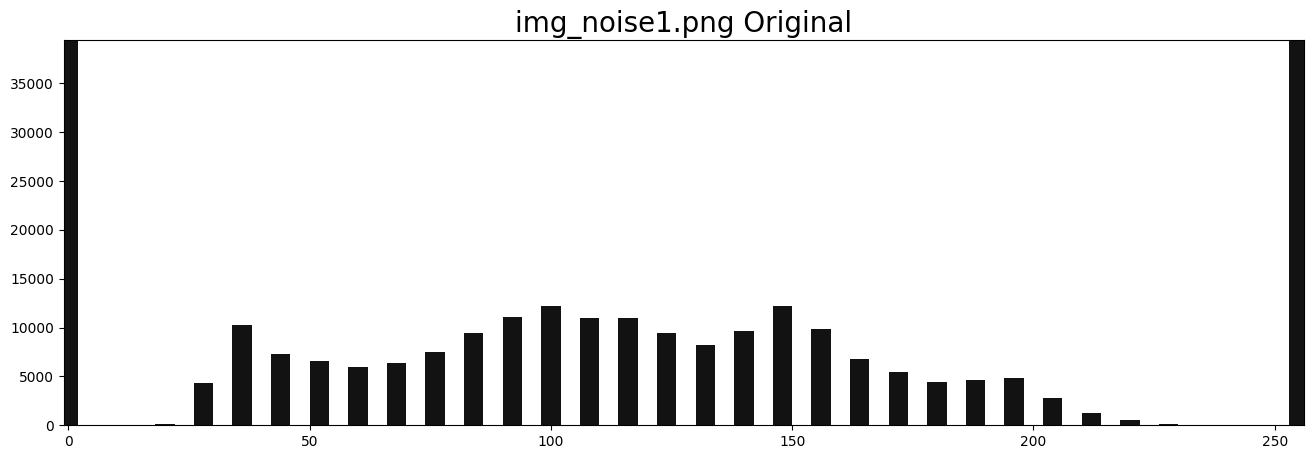
\includegraphics[height=5.3cm]{result_img/noise1_his.png}
%       \subcaption{Original Image}
%     \end{subfigure}
%     \begin{subfigure}{1\textwidth}
%       % 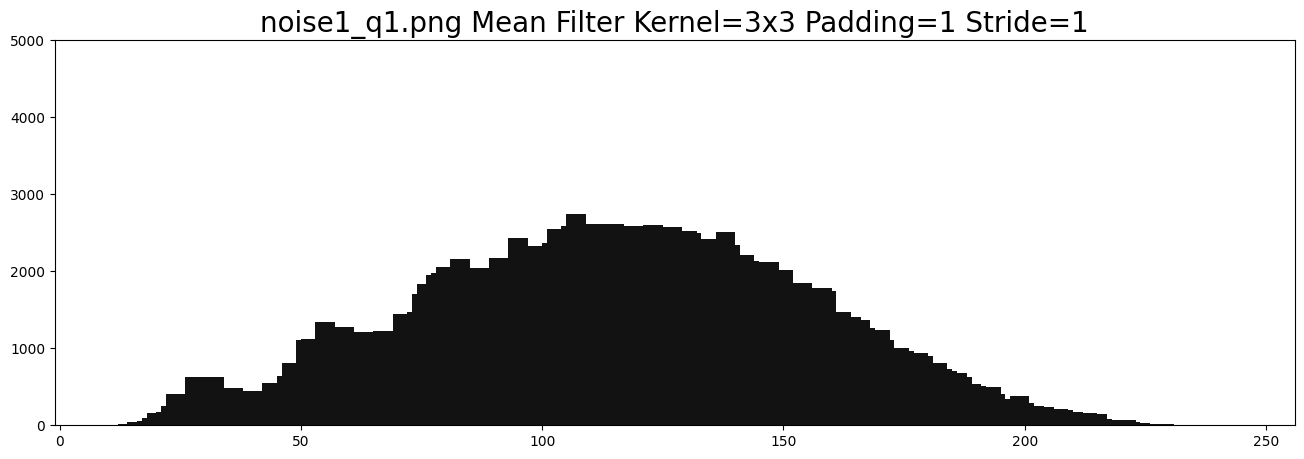
\includegraphics[height=5.3cm]{output/noise1_q1_K3P1_his.png}
%       \subcaption{Kernel = 3}
%     \end{subfigure}

%     \begin{subfigure}{1\textwidth}
%       % 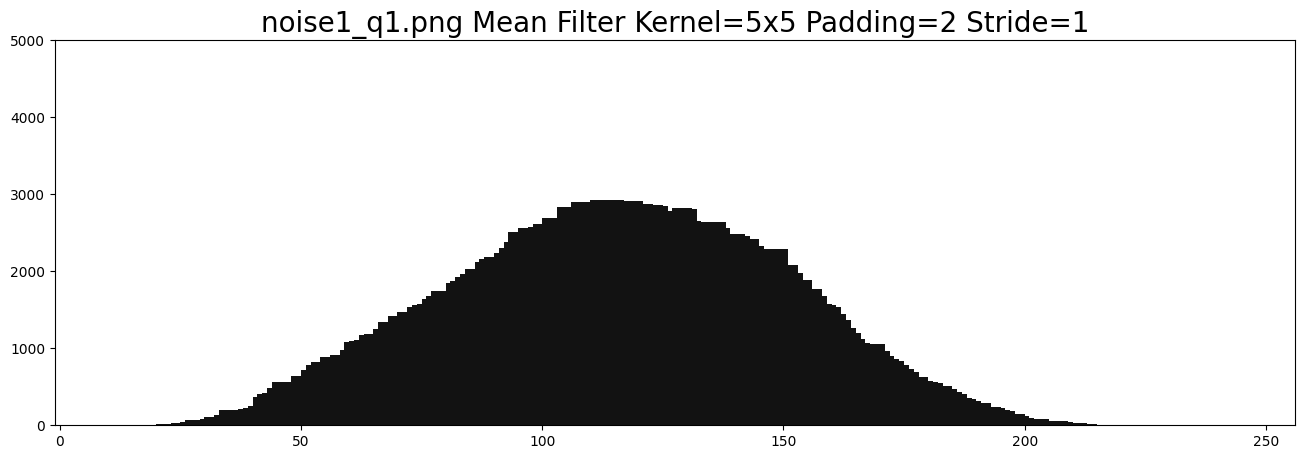
\includegraphics[height=5.3cm]{output/noise1_q1_K5P2_his.png}
%       \subcaption{Kernel = 5}
%     \end{subfigure}
%     \begin{subfigure}{1\textwidth}
%       % 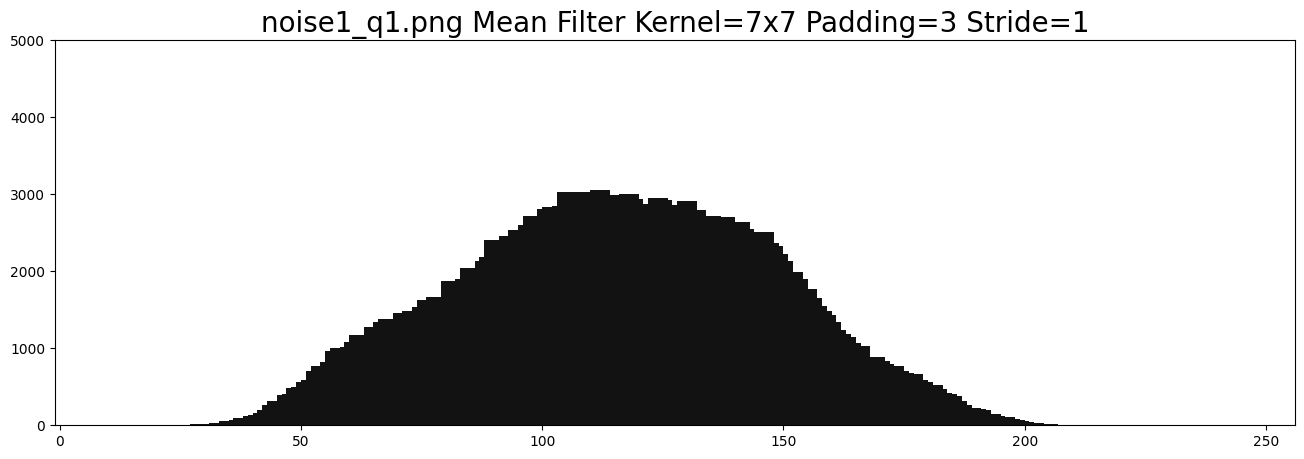
\includegraphics[height=5.3cm]{output/noise1_q1_K7P3_his.png}
%       \subcaption{Kernel = 7}
%     \end{subfigure}

%     \caption{Comparison of Histogram of noise1.png using Mean filter on different kernel size}
%     \label{fig:n1-mean-hist}
%   \end{minipage}
% \end{figure}
% \begin{figure}[!htb]
%   \begin{minipage}{\linewidth}
%     \centering
%     \begin{subfigure}{0.49\textwidth}
%       % 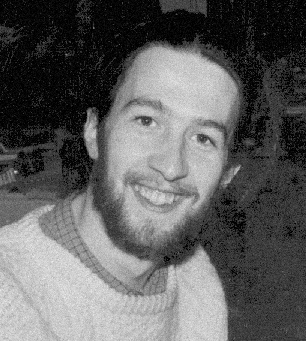
\includegraphics[width=\linewidth]{test_img/noise2.png}
%       \subcaption{Original Image}
%     \end{subfigure}
%     \begin{subfigure}{0.49\textwidth}
%       % 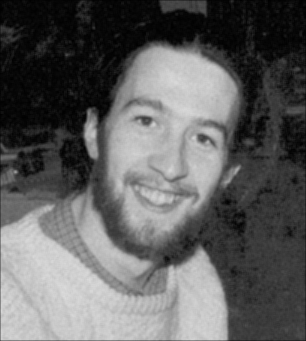
\includegraphics[width=\linewidth]{output/noise2_q1_K3P1.png}
%       \subcaption{Kernel = 3}
%     \end{subfigure}

%     \begin{subfigure}{0.49\textwidth}
%       % 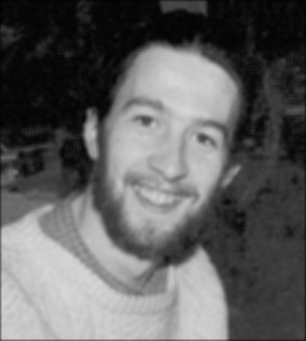
\includegraphics[width=\linewidth]{output/noise2_q1_K5P2.png}
%       \subcaption{Kernel = 5}
%     \end{subfigure}
%     \begin{subfigure}{0.49\textwidth}
%       % 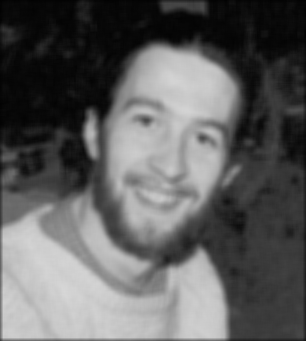
\includegraphics[width=\linewidth]{output/noise2_q1_K7P3.png}
%       \subcaption{Kernel = 7}
%     \end{subfigure}

%     \caption{Comparison of noise2.png using Mean filter on different kernel size}
%   \end{minipage}

% \end{figure}
% \begin{figure}[!htb]
%   \begin{minipage}{\linewidth}
%     \centering
%     \begin{subfigure}{1\textwidth}
%       % 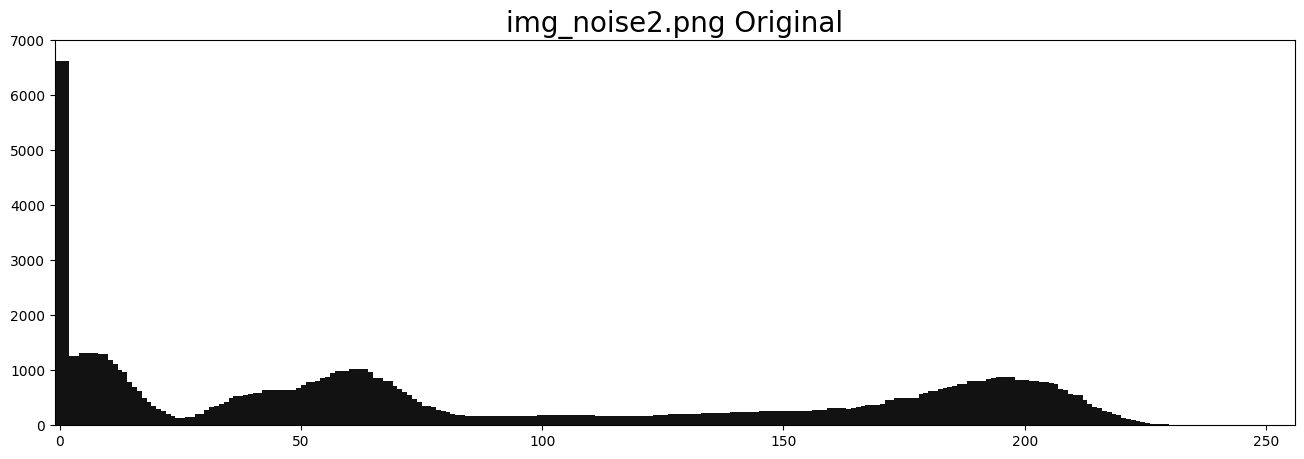
\includegraphics[height=5.3cm]{result_img/noise2_his.png}
%       \subcaption{Original Image}
%     \end{subfigure}
%     \begin{subfigure}{1\textwidth}
%       % 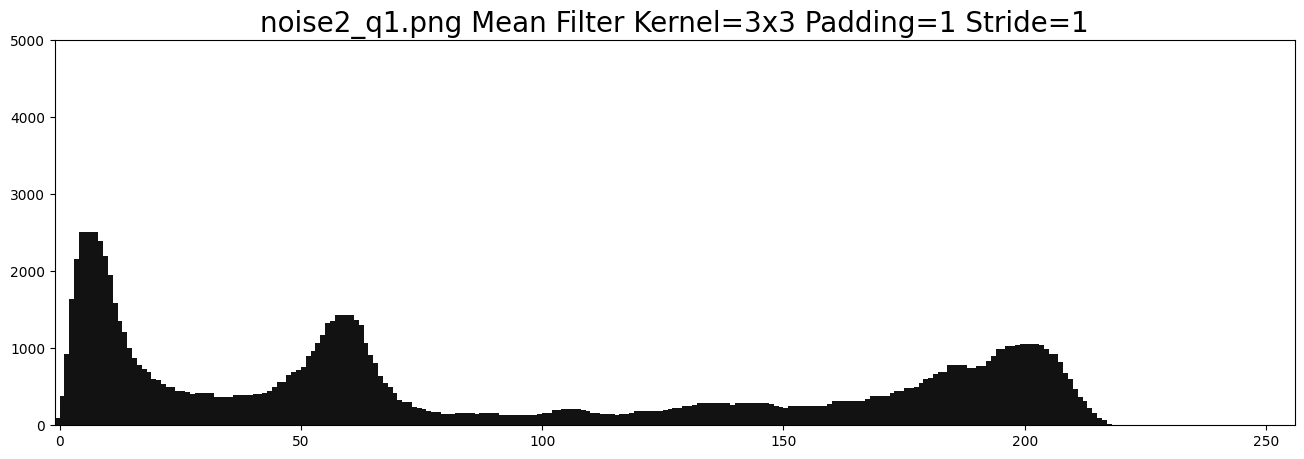
\includegraphics[height=5.3cm]{output/noise2_q1_K3P1_his.png}
%       \subcaption{Kernel = 3}
%     \end{subfigure}

%     \begin{subfigure}{1\textwidth}
%       % 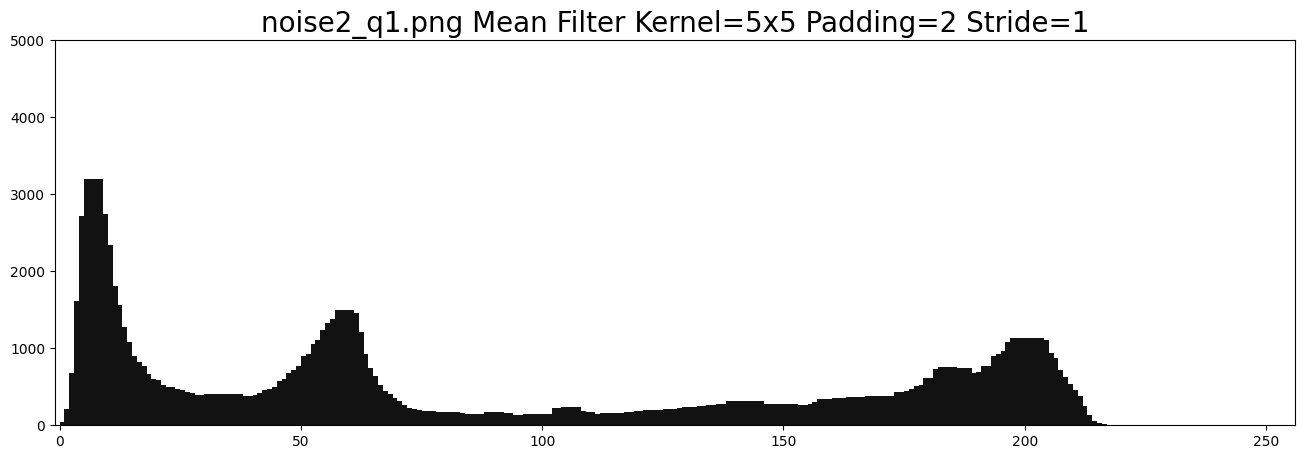
\includegraphics[height=5.3cm]{output/noise2_q1_K5P2_his.png}
%       \subcaption{Kernel = 5}
%     \end{subfigure}
%     \begin{subfigure}{1\textwidth}
%       % 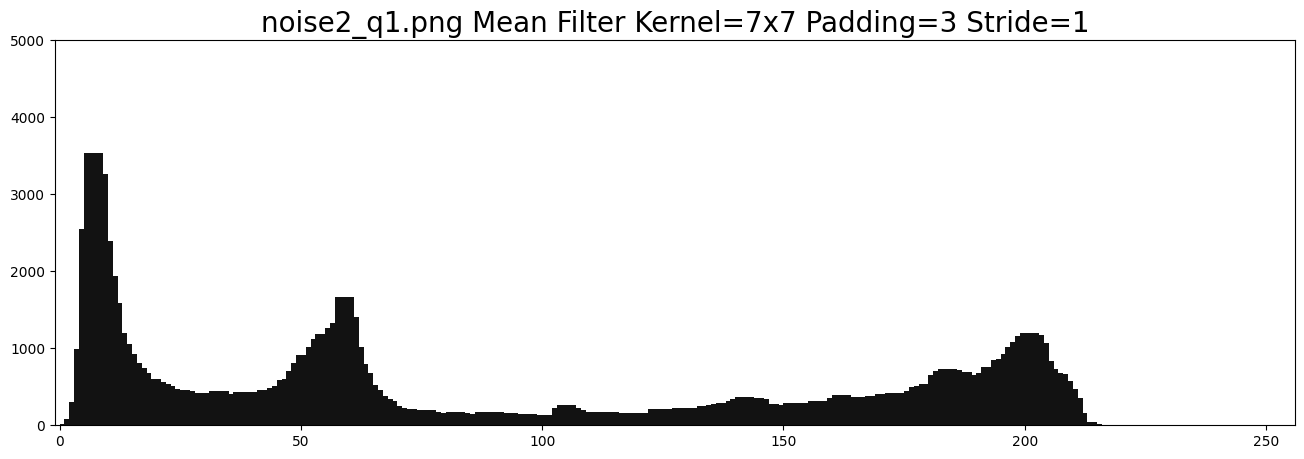
\includegraphics[height=5.3cm]{output/noise2_q1_K7P3_his.png}
%       \subcaption{Kernel = 7}
%     \end{subfigure}

%     \caption{Comparison of Histogram of noise2.png using Mean filter using different kernel size}
%     \label{fig:n2-mean-hist}
%   \end{minipage}
% \end{figure}
\clearpage


\subsection{Angle step in Hough Transform}
\paragraph*{}
Small angle step tends to over detect new line, while too high angle step will give inaccurate result as shown below.

\begin{figure}[!htb]
  \begin{minipage}{\linewidth}
    \centering
    \begin{subfigure}{0.49\textwidth}
      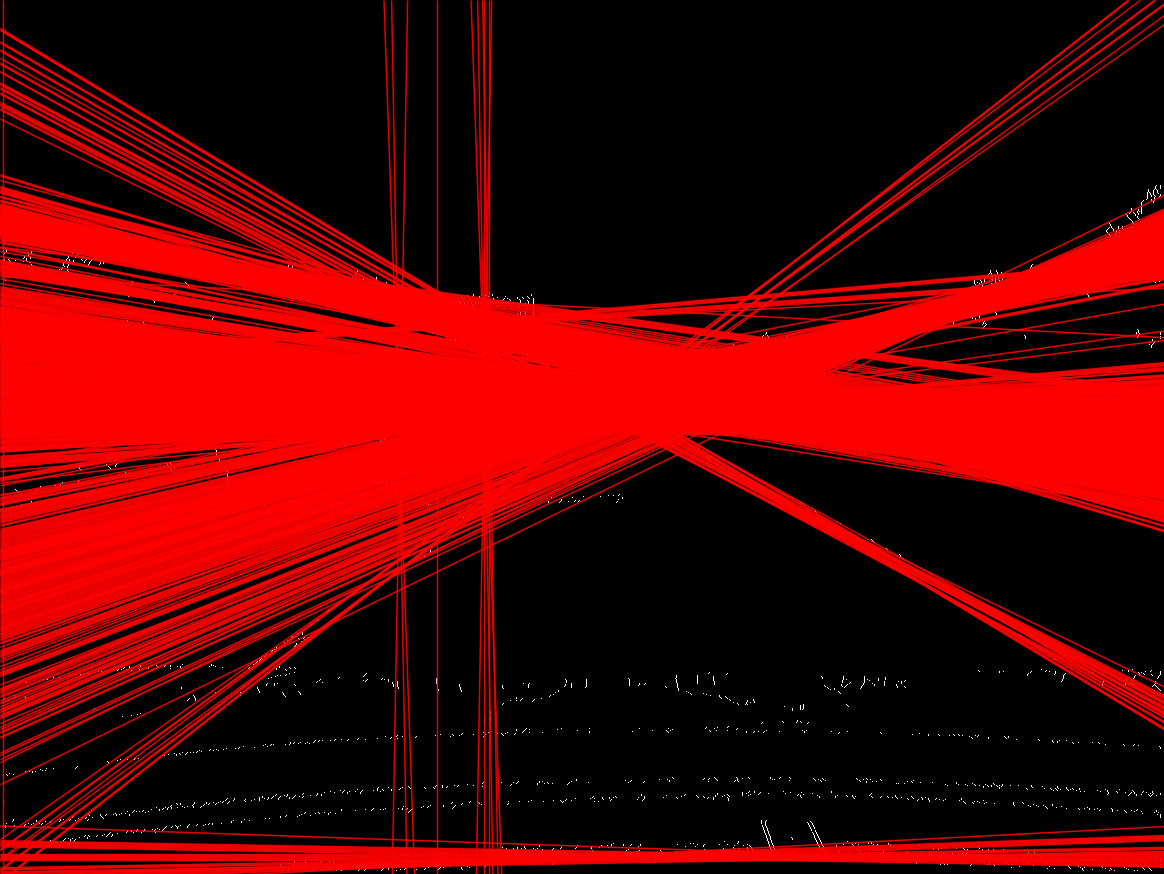
\includegraphics[width=\linewidth]{output/img2_q3_HOUGH_THETA_1_THRES_50.png}
      \subcaption{Theta = 1 deg}
    \end{subfigure}
    \begin{subfigure}{0.49\textwidth}
      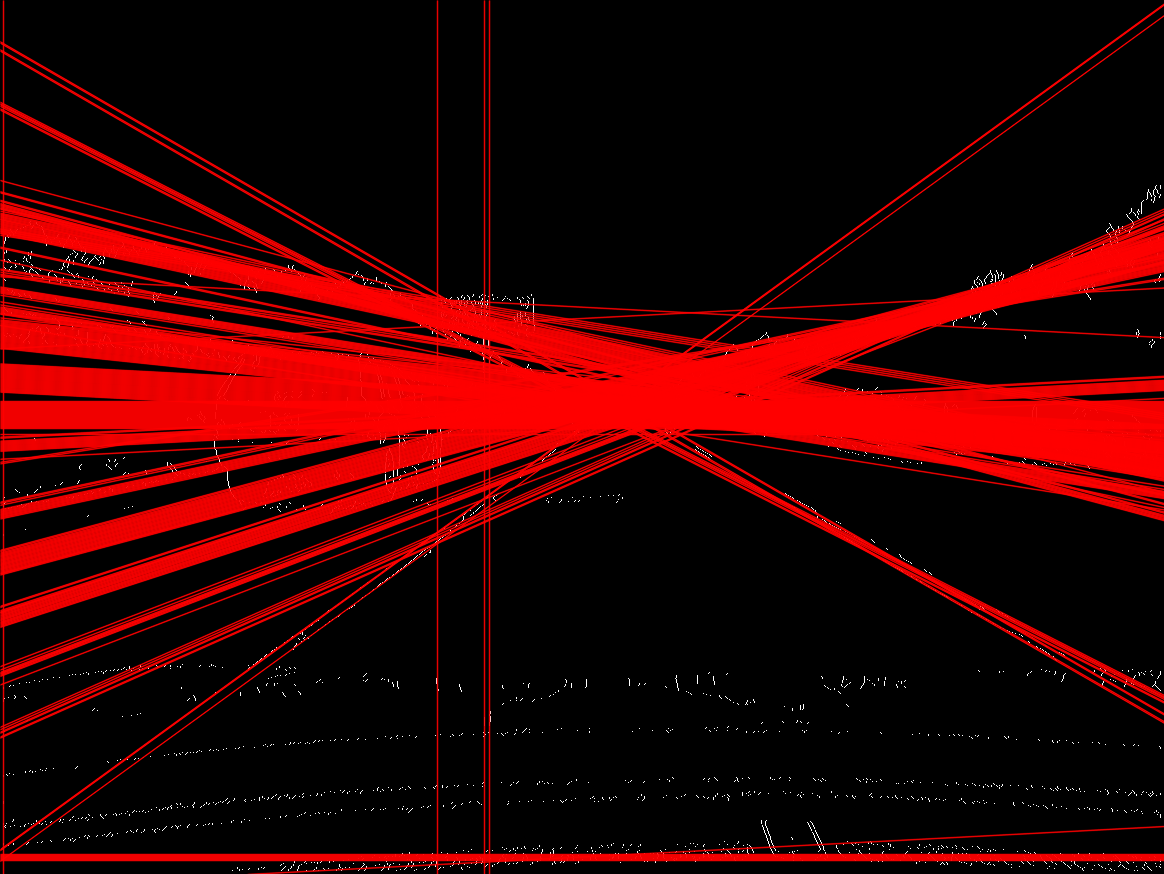
\includegraphics[width=\linewidth]{output/img2_q3_HOUGH_THETA_3_THRES_50.png}
      \subcaption{Theta = 3 deg}
    \end{subfigure}

    \begin{subfigure}{0.49\textwidth}
      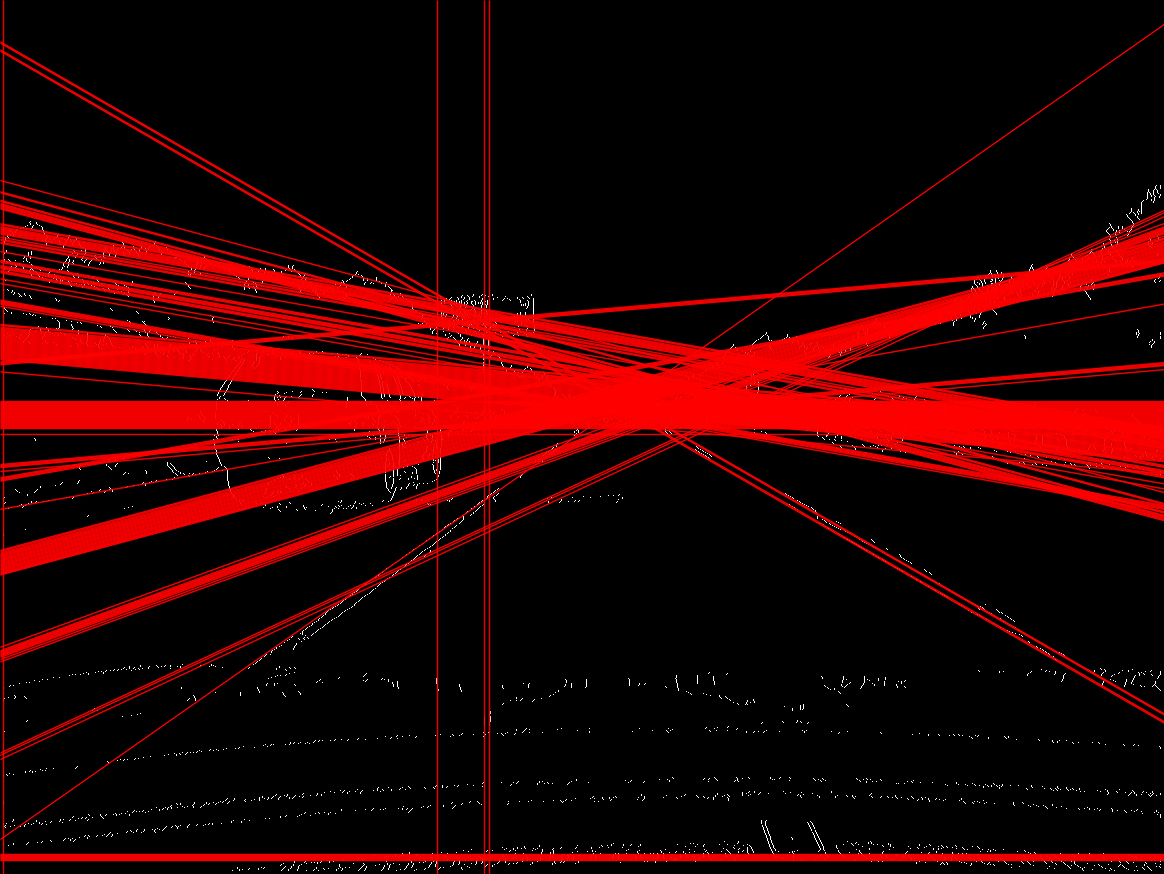
\includegraphics[width=\linewidth]{output/img2_q3_HOUGH_THETA_5_THRES_50.png}
      \subcaption{Theta = 5 deg}
    \end{subfigure}
    \begin{subfigure}{0.49\textwidth}
      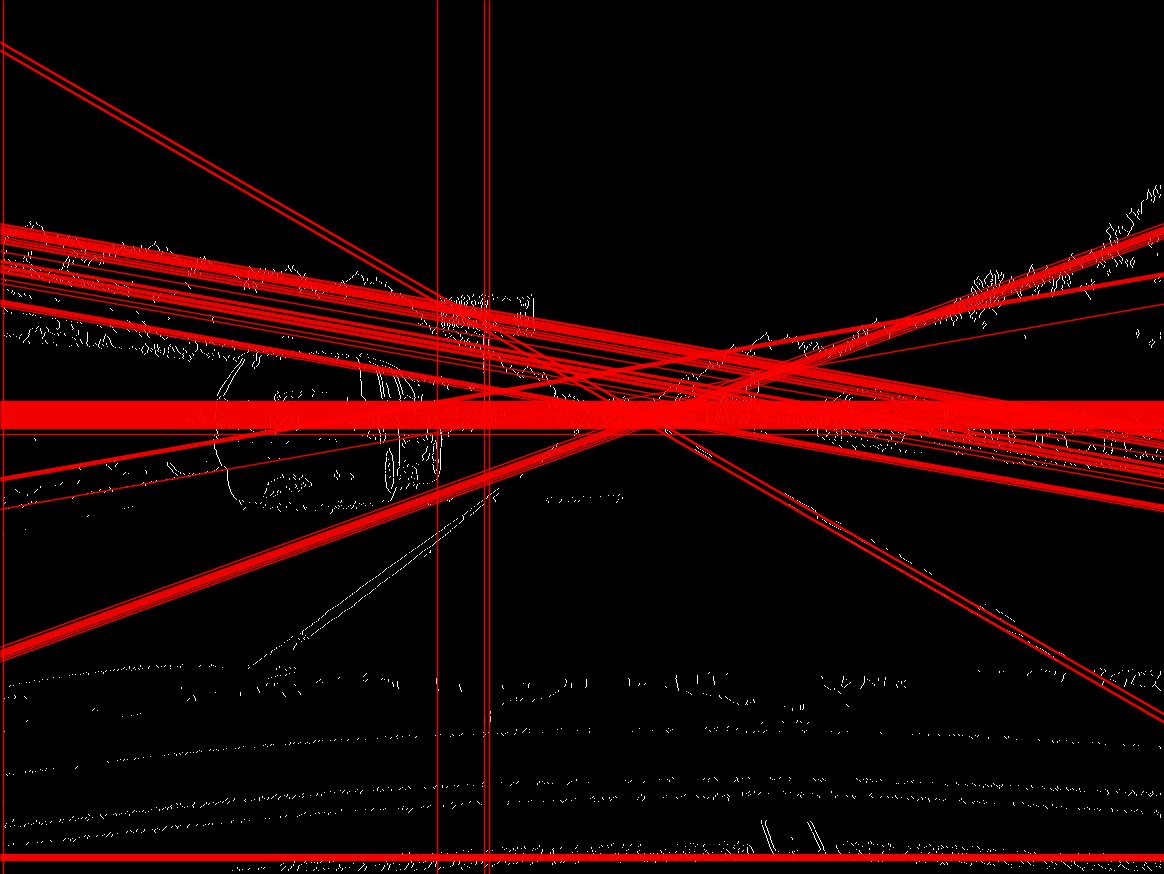
\includegraphics[width=\linewidth]{output/img2_q3_HOUGH_THETA_10_THRES_50.png}
      \subcaption{Theta = 10 deg}
    \end{subfigure}

    \caption{Comparison of Angle step affect line detection}
  \end{minipage}

\end{figure}
% \begin{figure}[!htb]
%   \begin{minipage}{\linewidth}
%     \centering
%     \begin{subfigure}{1\textwidth}
%       % 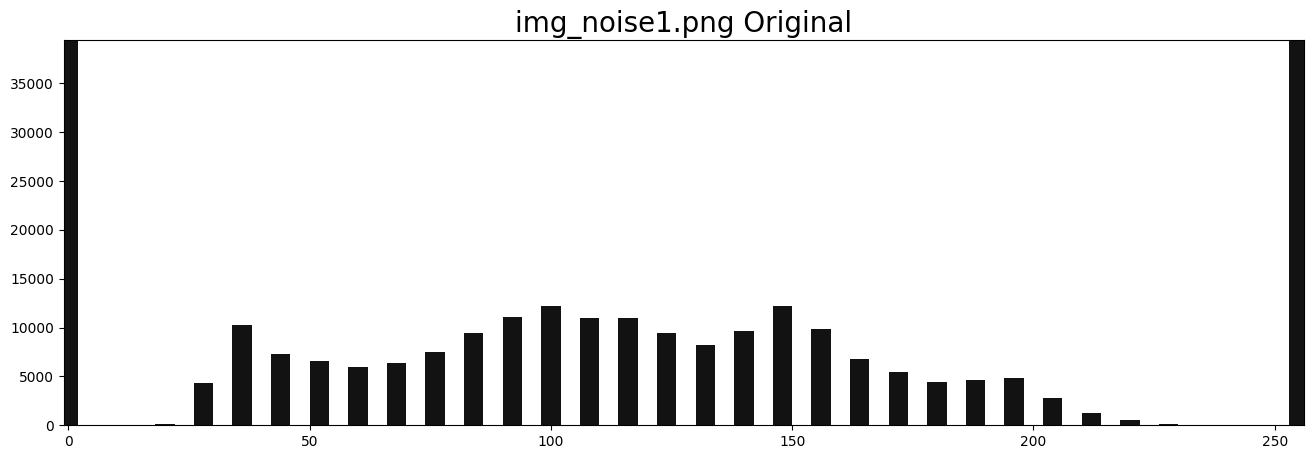
\includegraphics[height=5.3cm]{result_img/noise1_his.png}
%       \subcaption{Original Image}
%     \end{subfigure}
%     \begin{subfigure}{1\textwidth}
%       % 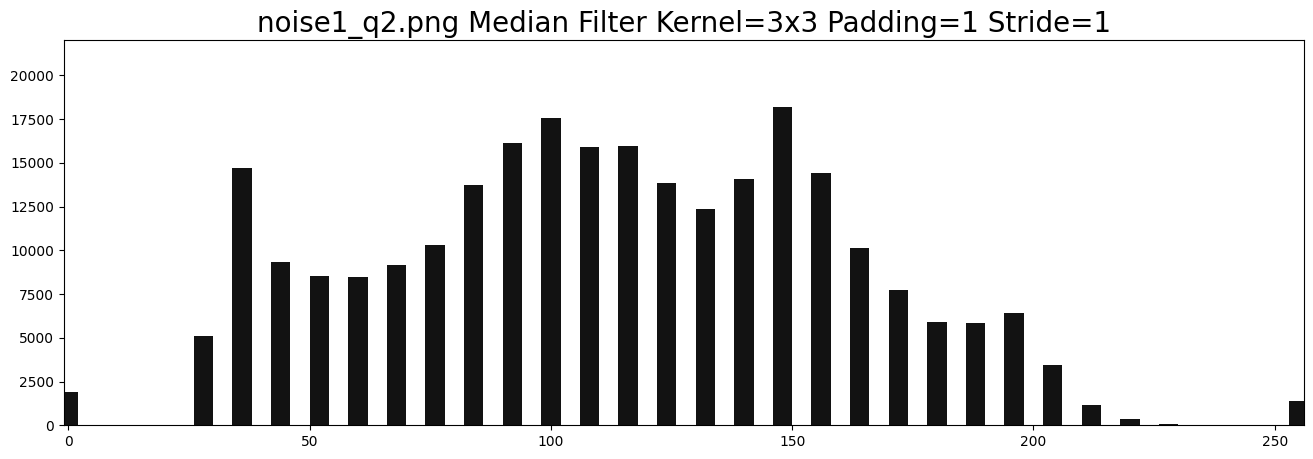
\includegraphics[height=5.3cm]{output/noise1_q2_K3P1_his.png}
%       \subcaption{Kernel = 3}
%     \end{subfigure}

%     \begin{subfigure}{1\textwidth}
%       % 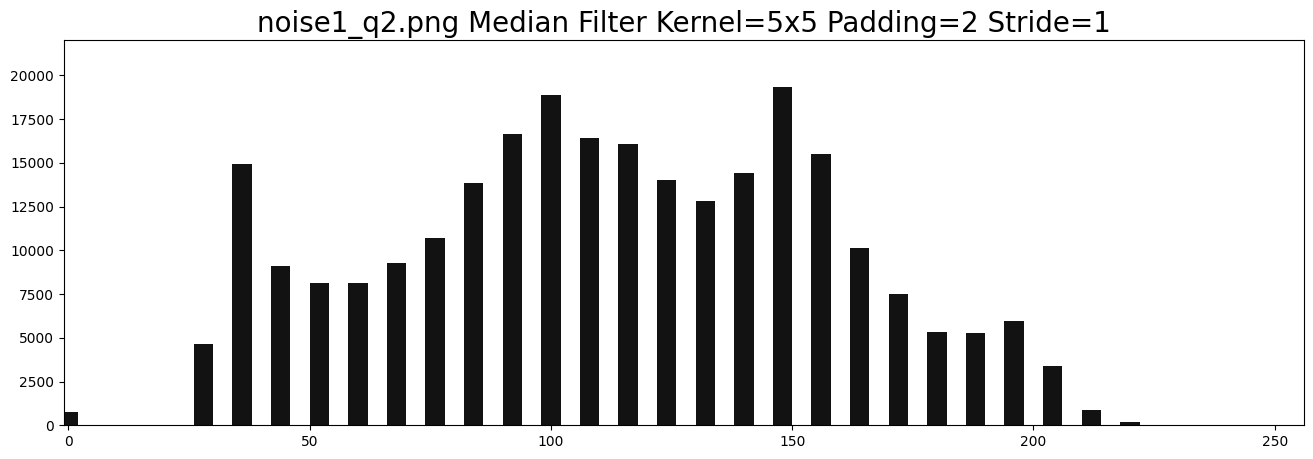
\includegraphics[height=5.3cm]{output/noise1_q2_K5P2_his.png}
%       \subcaption{Kernel = 5}
%     \end{subfigure}
%     \begin{subfigure}{1\textwidth}
%       % 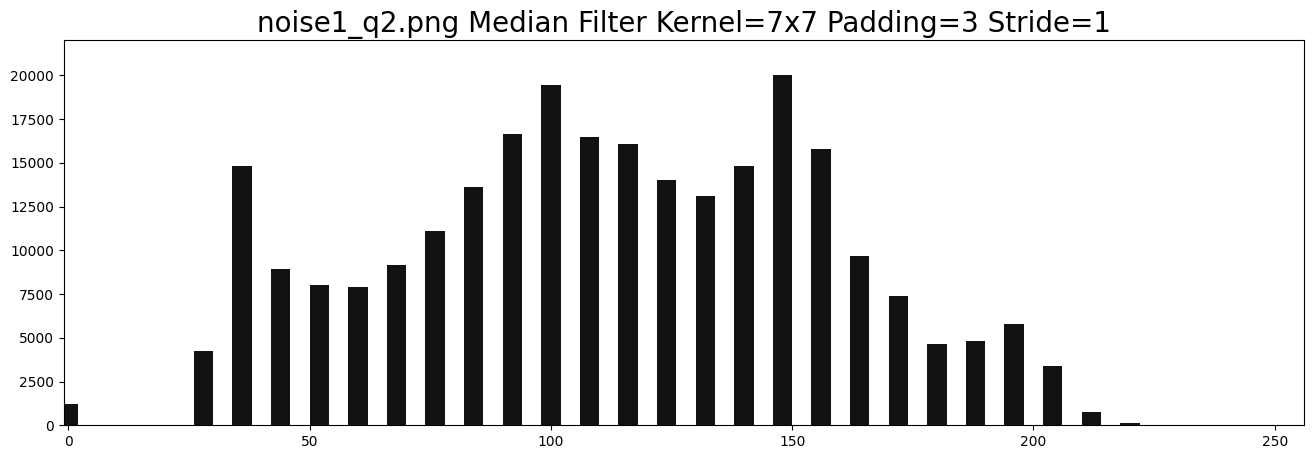
\includegraphics[height=5.3cm]{output/noise1_q2_K7P3_his.png}
%       \subcaption{Kernel = 7}
%     \end{subfigure}

%     \caption{Comparison of Histogram of noise1.png using Mean filter on different kernel size}
%     \label{fig:n1-median-hist}
%   \end{minipage}
% \end{figure}
% \begin{figure}[!htb]
%   \begin{minipage}{\linewidth}
%     \centering
%     \begin{subfigure}{0.49\textwidth}
%       % 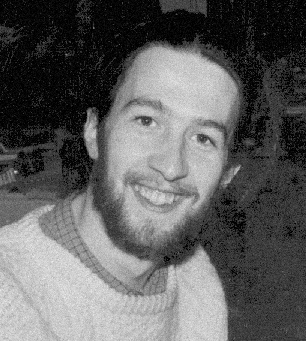
\includegraphics[width=\linewidth]{test_img/noise2.png}
%       \subcaption{Original Image}
%     \end{subfigure}
%     \begin{subfigure}{0.49\textwidth}
%       % 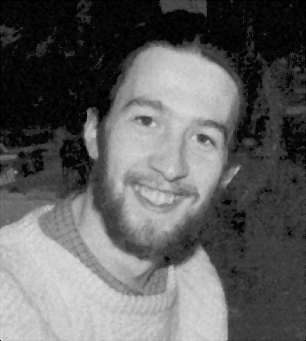
\includegraphics[width=\linewidth]{output/noise2_q2_K3P1.png}
%       \subcaption{Kernel = 3}
%     \end{subfigure}

%     \begin{subfigure}{0.49\textwidth}
%       % 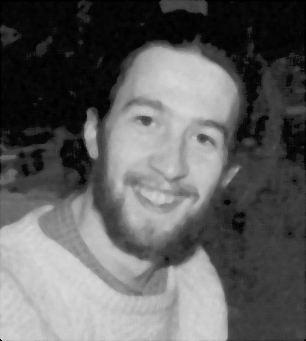
\includegraphics[width=\linewidth]{output/noise2_q2_K5P2.png}
%       \subcaption{Kernel = 5}
%     \end{subfigure}
%     \begin{subfigure}{0.49\textwidth}
%       % 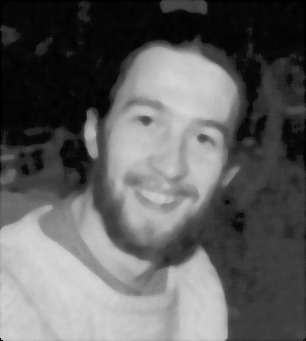
\includegraphics[width=\linewidth]{output/noise2_q2_K7P3.png}
%       \subcaption{Kernel = 7}
%     \end{subfigure}

%     \caption{Comparison of noise2.png using Mean filter on different kernel size}
%   \end{minipage}

% \end{figure}
% \begin{figure}[!htb]
%   \begin{minipage}{\linewidth}
%     \centering
%     \begin{subfigure}{1\textwidth}
%       % 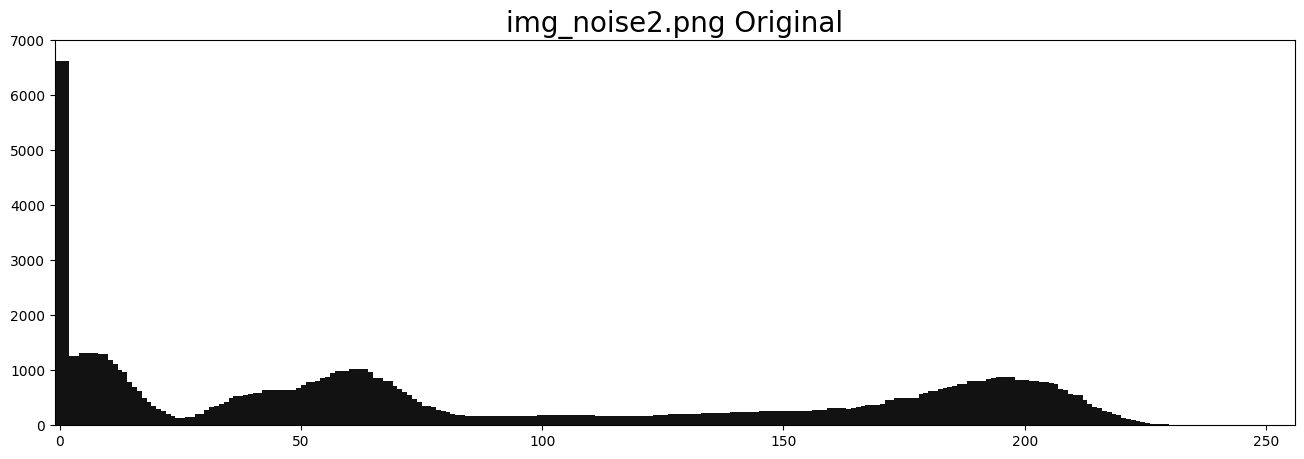
\includegraphics[height=5.3cm]{result_img/noise2_his.png}
%       \subcaption{Original Image}
%     \end{subfigure}
%     \begin{subfigure}{1\textwidth}
%       % 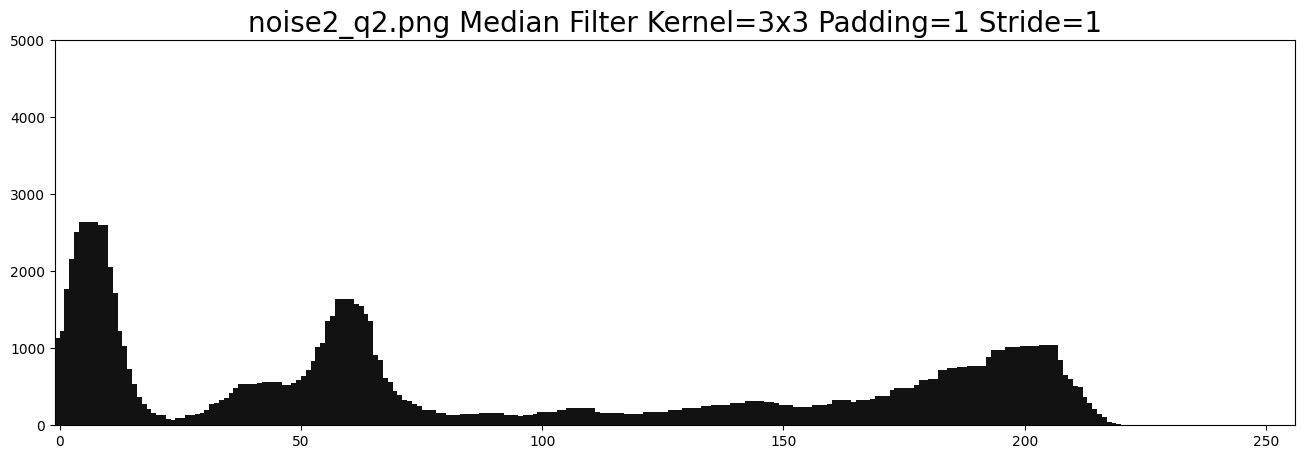
\includegraphics[height=5.3cm]{output/noise2_q2_K3P1_his.png}
%       \subcaption{Kernel = 3}
%     \end{subfigure}

%     \begin{subfigure}{1\textwidth}
%       % 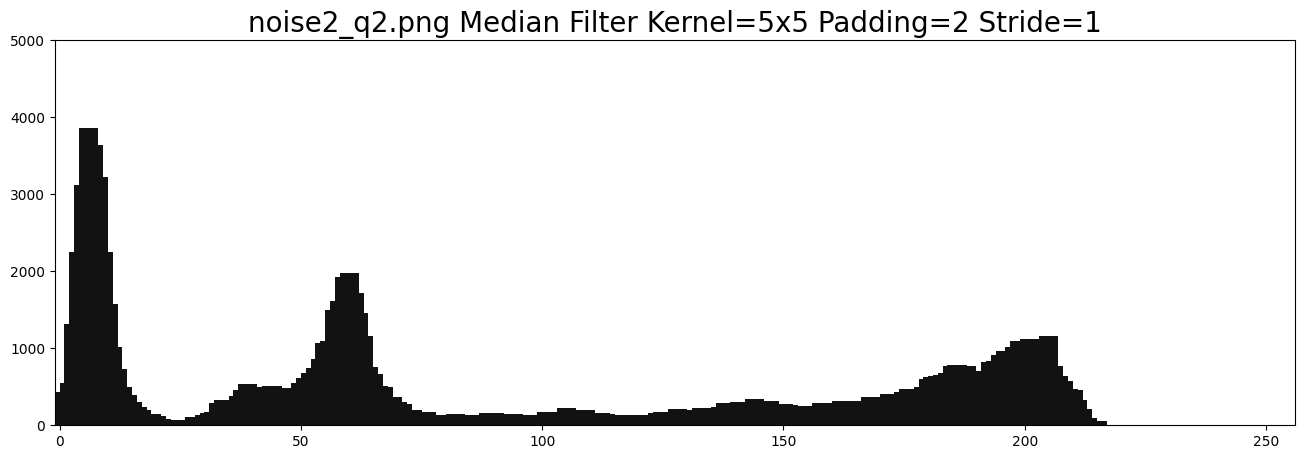
\includegraphics[height=5.3cm]{output/noise2_q2_K5P2_his.png}
%       \subcaption{Kernel = 5}
%     \end{subfigure}
%     \begin{subfigure}{1\textwidth}
%       % 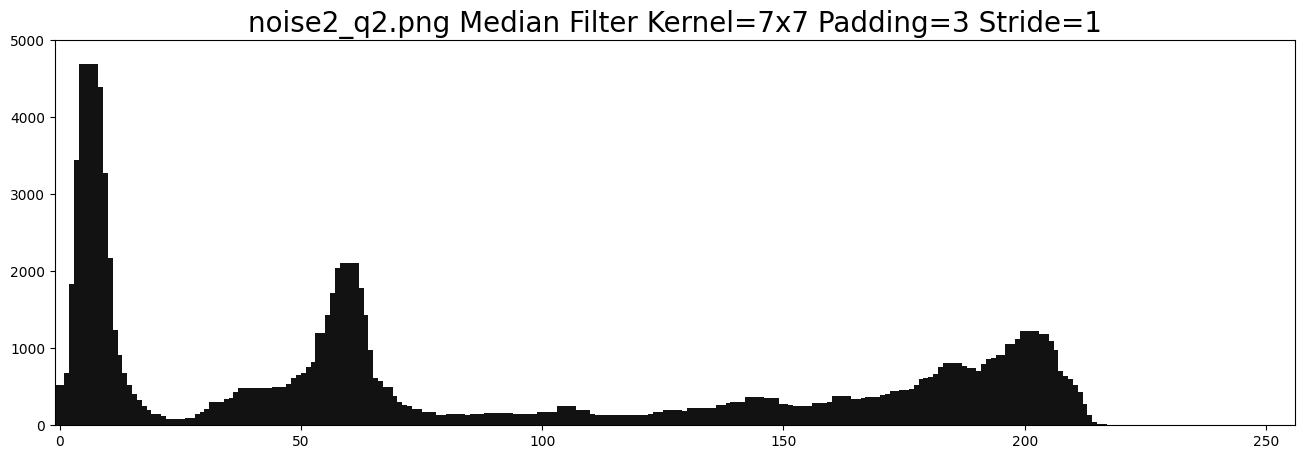
\includegraphics[height=5.3cm]{output/noise2_q2_K7P3_his.png}
%       \subcaption{Kernel = 7}
%     \end{subfigure}

%     \caption{Comparison of Histogram of noise2.png using Mean filter using different kernel size}
%     \label{fig:n2-median-hist}
%   \end{minipage}
% \end{figure}
\clearpage

\subsection{Choosing Filter}
\paragraph*{}Please be reminded that there is no single, complete formula that yields the best
result. For this case, prior knowledge about the line direction helps increase accuracy and reduce calculation complexity

\appendix
\chapter{Git Repository}

\verb|Git Repository: chinatip-l/computer-vision-lab-fall-2023| \\
URL: \url{https://github.com/chinatip-l/computer-vision-lab-fall-2023}

\chapter{Source Code: main.cpp}
\begin{lstlisting}
  #include <stdio.h>
  #include <opencv2/opencv.hpp>
  #include <unistd.h>
  #include <string.h>
  #include "include/func.hpp"
  
  #define MAX_LEN 250
  // // path for personal computer
  // #define BASE_PATH "/home/chinatip/work/computer_vision/homework3"
  
  // path for lab
  #define BASE_PATH "/home/chinatip/computer-vision-lab-fall-2023/homework3"
  #define SRC_PATH "test_img"
  #define OUT_PATH "output"
  
  // define file name, can uncomment to select the input
  #define FILENAME "img1"
  // #define FILENAME "img2"
  // #define FILENAME "img3"
  #define GAUSSIAN_FILT_SUFX "q1"
  #define CANNY_EDGE_SUFX "q2"
  #define HOUGH_SUFX "q3"
  #define KER_INFO_3 "K3P1"
  #define KER_INFO_5 "K5P2"
  #define KER_INFO_7 "K7P3"
  #define EXT "png"
  
  using namespace cv;
  
  Mat canvas;
  
  void appendImgToCanvas(Mat);
  
  int main(int argc, char **argv)
  {
  
      Mat og_img;
      char og_file[MAX_LEN] = "", out_file[MAX_LEN] = "";
      snprintf(og_file, MAX_LEN, "%s/%s/%s.%s", BASE_PATH, SRC_PATH, FILENAME, EXT);
  
      og_img = imread(og_file);
  
      if (!og_img.data)
      {
          printf("No image data \n");
          return -1;
      }
      else
      {
          printf("Original Img Size: w x h %d x %d\n", og_img.cols, og_img.rows);
      }
  
      appendImgToCanvas(og_img);
      Mat bw_img;
      bw_img = applyGreyscaleFilter(og_img);
  
      Mat res_img, selected_img;
      int kernel_size;
      float sigma;
      for (sigma = 0.5; sigma <= 2; sigma += 0.5)
      {
          for (kernel_size = 3; kernel_size <= 7; kernel_size += 2)
          {
              Mat gaussian_filter = createGaussianFilter(kernel_size, sigma);
              res_img = applyFilter(bw_img, gaussian_filter, 1, false);
              printf("Gaussian Filter Img Size: w x h %d x %d\n", res_img.cols, res_img.rows);
              snprintf(out_file, MAX_LEN, "%s/%s/%s_%s_K%d_SIG_%.1f.%s", BASE_PATH, OUT_PATH, FILENAME, GAUSSIAN_FILT_SUFX, kernel_size, sigma, EXT);
              imwrite(out_file, res_img);
              if (sigma == 1.0 && kernel_size == 5)
              {
                  selected_img = res_img.clone();
              }
          }
      }
      // appendImgToCanvas(selected_img);
  
      Mat sobelx;
      sobelx = applySobelX(selected_img);
      snprintf(out_file, MAX_LEN, "%s/%s/%s_%s_SOBEL_X.%s", BASE_PATH, OUT_PATH, FILENAME, CANNY_EDGE_SUFX, EXT);
      imwrite(out_file, sobelx);
      // appendImgToCanvas(sobelx);
  
      Mat sobely;
      sobely = applySobelY(selected_img);
      snprintf(out_file, MAX_LEN, "%s/%s/%s_%s_SOBEL_Y.%s", BASE_PATH, OUT_PATH, FILENAME, CANNY_EDGE_SUFX, EXT);
      imwrite(out_file, sobely);
      // appendImgToCanvas(sobely);
  
      Mat edge_strength;
      edge_strength = calculateEdgeStrength(sobelx, sobely);
      snprintf(out_file, MAX_LEN, "%s/%s/%s_%s_EDGE_STRENGTH.%s", BASE_PATH, OUT_PATH, FILENAME, CANNY_EDGE_SUFX, EXT);
      imwrite(out_file, edge_strength);
      // appendImgToCanvas(edge_strength);
  
      Mat edge_direction;
      edge_direction = calculateEdgeDirection(sobelx, sobely);
      snprintf(out_file, MAX_LEN, "%s/%s/%s_%s_EDGE_DIR.%s", BASE_PATH, OUT_PATH, FILENAME, CANNY_EDGE_SUFX, EXT);
      imwrite(out_file, edge_direction);
      // appendImgToCanvas(edge_direction);
  
      Mat nms;
      nms = calculateNonMaximumSuppression(edge_strength, edge_direction);
      snprintf(out_file, MAX_LEN, "%s/%s/%s_%s_NMS.%s", BASE_PATH, OUT_PATH, FILENAME, CANNY_EDGE_SUFX, EXT);
      imwrite(out_file, nms);
      // appendImgToCanvas(nms);
  
      Mat double_thresholed;
      double_thresholed = applyDoubleThresholding(nms, 10, 20);
      snprintf(out_file, MAX_LEN, "%s/%s/%s_%s_DTS.%s", BASE_PATH, OUT_PATH, FILENAME, CANNY_EDGE_SUFX, EXT);
      imwrite(out_file, double_thresholed);
      // appendImgToCanvas(double_thresholed);
  
      Mat hyst;
      hyst = applyHysteresis(double_thresholed);
      snprintf(out_file, MAX_LEN, "%s/%s/%s_%s_HYS.%s", BASE_PATH, OUT_PATH, FILENAME, CANNY_EDGE_SUFX, EXT);
      imwrite(out_file, hyst);
      appendImgToCanvas(hyst);
  
      // make a copy of hysteresis to use as result
      Mat hough = hyst.clone();
      std::vector<cv::Vec2f> ulines;
  
      // Parameters for Hough Transform
      float rho = 1; // distance resolution in pixels
      int theta_steps[] = {1, 3, 5, 10};
      int thresholds[] = { 35, 50, 75};
      for (int step_theta = 0; step_theta < 4; step_theta++)
      {
          for (int step_threshold = 0; step_threshold < 3; step_threshold++)
          {
              float theta = theta_steps[step_theta] * CV_PI / 180;
              int threshold = thresholds[step_threshold];
              // reset image
              hough = hyst.clone();
  
              // Apply Hough Transform
              applyHoughTransform(hyst, ulines, rho, theta, threshold);
  
              // Draw the lines on the original image
              for (size_t i = 0; i < ulines.size(); i++)
              {
                  float r = ulines[i][0], t = ulines[i][1];
                  double cos_t = std::cos(t), sin_t = std::sin(t);
                  double x0 = r * cos_t, y0 = r * sin_t;
                  double alpha = 2000; // length that the line will be drawn to cover the image
  
                  // Adjust the start and end points for the new origin at the center of the image
                  cv::Point pt1(cvRound(x0 + alpha * (-sin_t)), cvRound(y0 + alpha * cos_t));
                  cv::Point pt2(cvRound(x0 - alpha * (-sin_t)), cvRound(y0 - alpha * cos_t));
                  cv::line(hough, pt1, pt2, cv::Scalar(0, 0, 255), 1, cv::LINE_AA);
              }
              snprintf(out_file, MAX_LEN, "%s/%s/%s_%s_HOUGH_THETA_%d_THRES_%d.%s", BASE_PATH, OUT_PATH, FILENAME, HOUGH_SUFX,theta_steps[step_theta],threshold, EXT);
              imwrite(out_file, hough);
              if(threshold==75 && step_theta==0)
                  appendImgToCanvas(hough);
              // appendImgToCanvas(hough);
              ulines.clear();
          }
      }
  
      namedWindow("Original", WINDOW_AUTOSIZE);
  
      imshow("Original", canvas);
      waitKey(0);
      return 0;
  }
  
  void appendImgToCanvas(Mat img)
  {
      if (canvas.empty())
      {
          canvas = img;
      }
      else
      {
          Size s(canvas.cols + img.cols + 5, canvas.rows > img.rows ? canvas.rows : img.rows);
          size_t old_w = canvas.cols;
          copyMakeBorder(canvas, canvas, 0, 0, 0, img.cols + 5, BORDER_CONSTANT, Scalar(0, 0, 0, 0));
          img.copyTo(canvas(Rect(old_w + 5, 0, img.cols, img.rows)));
      }
  }  
\end{lstlisting}

\chapter{Source Code: func.hpp}
\begin{lstlisting}
#ifndef _FUNC_H_
#define _FUNC_H_

#include <opencv2/opencv.hpp>
#include <vector>

using namespace cv;

Mat applyGreyscaleFilter(Mat);
float calculateGaussian(int,int,float);

Mat createGaussianFilter(int,float);

Mat applyFilter(Mat , Mat , int ,bool);

Mat applySobelX(Mat);
Mat applySobelY(Mat);

Mat calculateEdgeStrength(Mat , Mat );
Mat calculateEdgeDirection(Mat , Mat );

int quantiseDirection(float);
Mat calculateNonMaximumSuppression(Mat , Mat ) ;

Mat applyDoubleThresholding(Mat ,int ,int );
Mat applyHysteresis(Mat);

void applyHoughTransform(cv::Mat, std::vector<cv::Vec2f>& , float , float , int );

#endif
\end{lstlisting}

\chapter{Source Code: func.cpp}
\begin{lstlisting}
#include "include/func.hpp"
#include <vector>
#include <cmath>
const double K_E = std::exp(1.0);

Mat applyGreyscaleFilter(Mat img)
{
    // Create New Image as Output Image
    Mat bw_img(img.size(), img.type());
    for (int j = 0; j < img.rows; j++)
    {
        for (int i = 0; i < img.cols; i++)
        {
            // Get the pixel value from the original image
            Vec3b brg_px = img.at<Vec3b>(j, i);

            // Normal average function ie. sum(xn)/n ;
            int b = (brg_px[0] + brg_px[1] + brg_px[2]) / 3;

            // Write back to every channel
            brg_px[0] = b;
            brg_px[1] = b;
            brg_px[2] = b;

            // Write to new image buffer
            bw_img.at<Vec3b>(j, i) = brg_px;
        }
    }
    // return the output image
    return bw_img;
}

float calculateGaussian(int x, int y, float sigma)
{
    return (1 / (CV_2PI * sigma * sigma)) * (powf32(K_E, -1 * ((x * x) + (y * y)) / (2 * sigma * sigma)));
}

Mat createGaussianFilter(int size, float sigma)
{
    int center = size / 2;
    Mat kernel = Mat::zeros(size, size, CV_32F);
    for (int j = 0; j < kernel.rows; j++)
    {
        for (int i = 0; i < kernel.cols; i++)
        {
            kernel.at<float>(j, i) = calculateGaussian(i - center, j - center, sigma);
        }
    }
    return kernel;
}

Mat applyFilter(Mat img, Mat kernel, int stride, bool suppress_border)
{

    // calculate kernel offset ie. number of pixel before and
    // after since the target pixel will be the center of
    // matrix,
    // in order to get the neighbour pixel with size of kernel
    // size, offset will be applied for both before, and after
    // the target pixel
    // example
    // width = 5 => offset = (int)5/2 = 2;
    // px   ... k   n-offset    ... n   ... n+offset    k
    int ker_x_offset = kernel.cols / 2;
    int ker_y_offset = kernel.rows / 2;

    int padding = ker_x_offset;

    // get kernel size
    int ker_w = kernel.cols;
    int ker_h = kernel.rows;

    // calculate output image size
    int out_w = ((img.cols + (2 * padding) - kernel.cols) / stride) + 1;
    int out_h = ((img.rows + (2 * padding) - kernel.rows) / stride) + 1;

    // create intermediate buffer and add padding, size is
    // w+(2*padding),h+(2*padding) then copy the content
    // of image to the buffer
    Mat padded;
    padded = Mat::zeros(img.rows + (2 * padding), img.cols + (2 * padding), CV_32SC3);
    int dtype = img.type();

    // here, we convert data type while copy to make it compatible
    // for higher precision computation
    // check if input is uint8 or int 32
    // if uint8 then we will channel-wise copy to padded buffer
    // due to different data alignment
    // if int38 then we will pixel-wise copy to padded buffer
    switch (dtype)
    {
    case CV_32SC3:
        for (int j = 0; j < img.rows; j++)
        {
            for (int i = 0; i < img.cols; i++)
            {
                padded.at<Vec3i>(j + padding, i + padding) = img.at<Vec3i>(j, i);
            }
        }
        break;
    case CV_8UC3:
        for (int j = 0; j < img.rows; j++)
        {
            for (int i = 0; i < img.cols; i++)
            {
                for (int k = 0; k < 3; k++)
                {
                    padded.at<Vec3i>(j + padding, i + padding)[k] = img.at<Vec3b>(j, i)[k];
                }
            }
        }
        break;
    default:
        break;
    }

    // create output buffer with calculated output size
    // data type need to be vector of signed int 32 bit
    // in case negative data is possible, this can help
    // preserve information through the convolution process
    // and rasterise to 8 bit at the last step
    Mat img_res = Mat::zeros(out_h, out_w, CV_32SC3);

    Vec3i res(0, 0, 0);

    // iterate over the size of input image
    for (int img_j = 0; img_j < img.rows; img_j += stride)
    {
        for (int img_i = 0; img_i < img.cols; img_i += stride)
        {
            // check if it is a border and suppress border if selected
            if (img_i < ker_w || img_j < ker_h || img_i > img.cols - ker_h - 1 || img_j > img.rows - ker_h - 1)
            {
                if (suppress_border)
                {
                    res = Vec3i(0, 0, 0);
                    img_res.at<Vec3i>((img_j) / stride, (img_i) / stride) = res;
                    continue;
                }
            }

            // get windowed matrix from the padded buffer with
            // the size of kernel size, and target pixel is in
            // the center of windowed matrix
            Mat windowed = padded(Rect(img_i, img_j, ker_w, ker_h));
            res = Vec3i(0, 0, 0);
            float tmp = 0;
            float tmp1 = 0;
            float tmp2 = 0;
            float tmp3 = 0;

            // item-wise multiply windowed matrix with kernel
            // matrix and summarise
            for (int ker_j = 0; ker_j < kernel.rows; ker_j++)
            {
                for (int ker_i = 0; ker_i < kernel.cols; ker_i++)
                {
                    Vec3b t = windowed.at<Vec3i>(ker_j, ker_i);
                    float k = kernel.at<float>(ker_j, ker_i);
                    tmp += (t[0] * k);
                    tmp1 += (t[0] * k);
                    tmp2 += (t[1] * k);
                    tmp3 += (t[2] * k);
                }
            }
            res[0] = tmp1;
            res[1] = tmp2;
            res[2] = tmp3;

            // write to output buffer
            img_res.at<Vec3i>((img_j) / stride, (img_i) / stride) = res;
        }
    }
    // return the output image
    return img_res;
}

Mat applySobelX(Mat img_in)
{
    float c_sobelX[] = {-1, 0, 1,
                        -2, 0, 2,
                        -1, 0, 1};
    Mat sobelX(3, 3, CV_32F, c_sobelX);
    Mat result = applyFilter(img_in, sobelX, 1, true);
    return result;
}

Mat applySobelY(Mat img_in)
{
    float c_sobelY[] = {-1, -2, -1,
                          0,  0,  0,
                          1,  2,  1};
    Mat sobelY(3, 3, CV_32F, c_sobelY);
    Mat result = applyFilter(img_in, sobelY, 1, true);
    return result;
}

Mat calculateEdgeStrength(Mat x, Mat y)
{
    Mat strength = Mat::zeros(x.rows, x.cols, CV_32FC3);
    float tmp = 0;
    for (int j = 0; j < strength.rows; j += 1)
    {
        for (int i = 0; i < strength.cols; i += 1)
        {
            for (int k = 0; k < 3; k++)
            {
                // Strength of pixel is calculated by
                // sqrt(gx^2 + gy^2)
                tmp = (x.at<Vec3i>(j, i)[k] * x.at<Vec3i>(j, i)[k]) + (y.at<Vec3i>(j, i)[k] * y.at<Vec3i>(j, i)[k]);
                strength.at<Vec3f>(j, i)[k] = sqrtf32(tmp);
            }
        }
    }

    return strength;
}

Mat calculateEdgeDirection(Mat x, Mat y)
{
    Mat direction = Mat::zeros(x.rows, x.cols, CV_32FC3);
    for (int j = 0; j < direction.rows; j += 1)
    {
        for (int i = 0; i < direction.cols; i += 1)
        {
            for (int k = 0; k < 3; k++)
            {
                // direction of pixel is calculated by
                // atan(y/x)
                direction.at<Vec3f>(j, i)[k] = atan2f32(y.at<Vec3f>(j, i)[k], x.at<Vec3f>(j, i)[k]) * 10;
            }
        }
    }
    return direction;
}

int quantiseDirection(float angle)
{
    // convert radiant to degree
    angle = angle * 180 / CV_PI;

    // quantise to 4 axes 
    if ((angle >= 0 && angle < 22.5) || (angle >= 157.5 && angle <= 180))
    {
        return 0;
    }
    else if (angle >= 22.5 && angle < 67.5)
    {
        return 45;
    }
    else if (angle >= 67.5 && angle < 112.5)
    {
        return 90;
    }
    else if (angle >= 112.5 && angle < 157.5)
    {
        return 135;
    }
    else
    {
        return 0;
    }
}

Mat calculateNonMaximumSuppression(cv::Mat strength, cv::Mat direction)
{
    // Create a zero-initialized matrix with the same size as the input, to store the result
    Mat res = Mat::zeros(strength.rows, strength.cols, CV_32SC3);

    // Iterate over the image, avoiding the borders (as the algorithm needs neighboring pixels)
    for (int j = 1; j < strength.rows - 1; j++)
    {
        for (int i = 1; i < strength.cols - 1; i++)
        {
            // Iterate over each channel (assuming a 3-channel image)
            for (int k = 0; k < 3; k++)
            {
                // Quantize the direction to one of the four possible angles (0, 45, 90, 135)
                int dir = quantiseDirection(direction.at<Vec3f>(j, i)[k]);

                // Retrieve the strength of the neighboring pixels in all 8 directions
                float neighbour_UL = strength.at<Vec3f>(j - 1, i - 1)[k];
                float neighbour_UM = strength.at<Vec3f>(j - 1, i)[k];
                float neighbour_UR = strength.at<Vec3f>(j - 1, i + 1)[k];
                float neighbour_ML = strength.at<Vec3f>(j, i - 1)[k];
                float neighbour_CC = strength.at<Vec3f>(j, i)[k]; // Current pixel
                float neighbour_MR = strength.at<Vec3f>(j, i + 1)[k];
                float neighbour_DL = strength.at<Vec3f>(j + 1, i - 1)[k];
                float neighbour_DM = strength.at<Vec3f>(j + 1, i)[k];
                float neighbour_DR = strength.at<Vec3f>(j + 1, i + 1)[k];

                // Initially set the result pixel to the current strength
                res.at<Vec3i>(j, i)[k] = (int)neighbour_CC;

                // Depending on the quantized direction, suppress non-maximum pixels
                // by setting them to zero if they are not the local maxima along the gradient direction
                switch (dir)
                {
                case 0:
                    if (neighbour_CC <= neighbour_ML || neighbour_CC <= neighbour_MR)
                        res.at<Vec3f>(j, i)[k] = 0;
                    break;
                case 45:
                    if (neighbour_CC <= neighbour_UR || neighbour_CC <= neighbour_DL)
                        res.at<Vec3f>(j, i)[k] = 0;
                    break;
                case 90:
                    if (neighbour_CC <= neighbour_UM || neighbour_CC <= neighbour_DM)
                        res.at<Vec3f>(j, i)[k] = 0;
                    break;
                case 135:
                    if (neighbour_CC <= neighbour_UL || neighbour_CC <= neighbour_DR)
                        res.at<Vec3f>(j, i)[k] = 0;
                    break;
                }
            }
        }
    }

    // Return the resulting image after non-maximum suppression
    return res;
}

Mat applyDoubleThresholding(Mat input, int thres_low, int thres_high)
{
    // Create a zero-initialized matrix with the same size as the input, to store the result
    Mat res = Mat::zeros(input.rows, input.cols, CV_8UC3);

    // Temporary variable to store the intensity of the current pixel
    int tmp = 0;

    // Iterate over the image, avoiding the borders
    for (int j = 1; j < input.rows - 1; j++)
    {
        for (int i = 1; i < input.cols - 1; i++)
        {
            // Iterate over each channel of the pixel
            for (int k = 0; k < 3; k++)
            {
                // Get the intensity value of the current pixel
                tmp = input.at<Vec3i>(j, i)[k];

                // If the intensity is higher than the high threshold, mark it as a strong edge (255)
                if (tmp >= thres_high)
                {
                    res.at<Vec3b>(j, i)[k] = 255;
                }
                // If the intensity is lower than the low threshold, suppress it (0)
                else if (tmp < thres_low)
                {
                    res.at<Vec3b>(j, i)[k] = 0;
                }
                // If the intensity is between the low and high thresholds, mark it as a weak edge (128)
                else
                {
                    res.at<Vec3b>(j, i)[k] = 128;
                }
            }
        }
    }

    // Return the resulting image after double thresholding
    return res;
}

Mat applyHysteresis(Mat input)
{
    // Clone the input image to preserve the original and work on a copy
    Mat res = input.clone();

    // Define constants for weak and strong edge values
    int WEAK = 128, STRONG = 255;

    // Iterate over the image, avoiding the borders
    for (int j = 1; j < res.rows - 1; j++)
    {
        for (int i = 1; i < res.cols - 1; i++)
        {
            // Iterate over each channel of the pixel
            for (int k = 0; k < 3; k++)
            {
                // Check if the current pixel is a weak edge
                if (res.at<Vec3b>(j, i)[k] == WEAK)
                {
                    // Initialize a flag to check if the weak edge is connected to a strong edge
                    bool connected = false;

                    // Check the 8 neighboring pixels to see if any of them is a strong edge
                    for (int dj = -1; dj <= 1; ++dj)
                    {
                        for (int di = -1; di <= 1; ++di)
                        {
                            // Skip the current pixel
                            if (di == 0 && dj == 0)
                                continue;

                            // If a strong edge is found in the neighborhood, set the flag
                            if (res.at<Vec3b>(j + dj, i + di)[k] == STRONG)
                            {
                                connected = true;
                                break;
                            }
                        }
                        if (connected)
                            break;
                    }

                    // If the weak edge is connected to a strong edge, strengthen it; otherwise, suppress it
                    res.at<Vec3b>(j, i)[k] = connected ? STRONG : 0;
                }
            }
        }
    }

    // Return the resulting image after applying hysteresis
    return res;
}


void applyHoughTransform(cv::Mat edges, std::vector<cv::Vec2f> &lines, float rho, float theta, int threshold)
{
    // Get the dimensions of the edges image
    int width = edges.cols;
    int height = edges.rows;

    // Calculate the maximum distance (rho) possible in the image
    int rho_max = (int)(std::sqrt(width * width + height * height));

    // Calculate the maximum number of bins for theta
    int theta_max = (int)(CV_PI / theta);

    // Create the accumulator matrix initialized to zero
    cv::Mat accum = cv::Mat::zeros(2 * rho_max, theta_max, CV_32S);

    // Iterate over the pixels of the edges image
    for (int y = 0; y < edges.rows; y++)
    {
        for (int x = 0; x < edges.cols; x++)
        {
            // Check if the current pixel is part of an edge
            if (edges.at<Vec3b>(y, x)[0] > 0)
            {
                // For each angle theta, calculate the corresponding rho value
                for (int t = 0; t < theta_max; t++)
                {
                    double current_theta = (t * theta);

                    // Calculate rho for the current (x, y) point and theta
                    double rho_val = cvRound((x * std::cos(current_theta)) + (y * std::sin(current_theta)));
                    int rho_index = (int)((rho_val / rho) + rho_max);

                    // Increment the accumulator's bin if the index is valid
                    if (rho_index >= 0 && rho_index < 2 * rho_max)
                    {
                        accum.at<int>(rho_index, t)++;
                    }
                }
            }
        }
    }

    // Iterate over the accumulator to find local maxima (lines)
    for (int r = 0; r < 2 * rho_max; r++)
    {
        for (int t = 0; t < theta_max; t++)
        {
            // If the bin's value is above the threshold, it is considered a line
            if (accum.at<int>(r, t) >= threshold)
            {
                // Convert (rho, theta) from accumulator space to image space and add to the lines vector
                lines.push_back(cv::Vec2f(r * rho - rho_max, t * theta));
            }
        }
    }
}
\end{lstlisting}

\chapter{Result Images}
\begin{figure}[!htb]
  \centering
  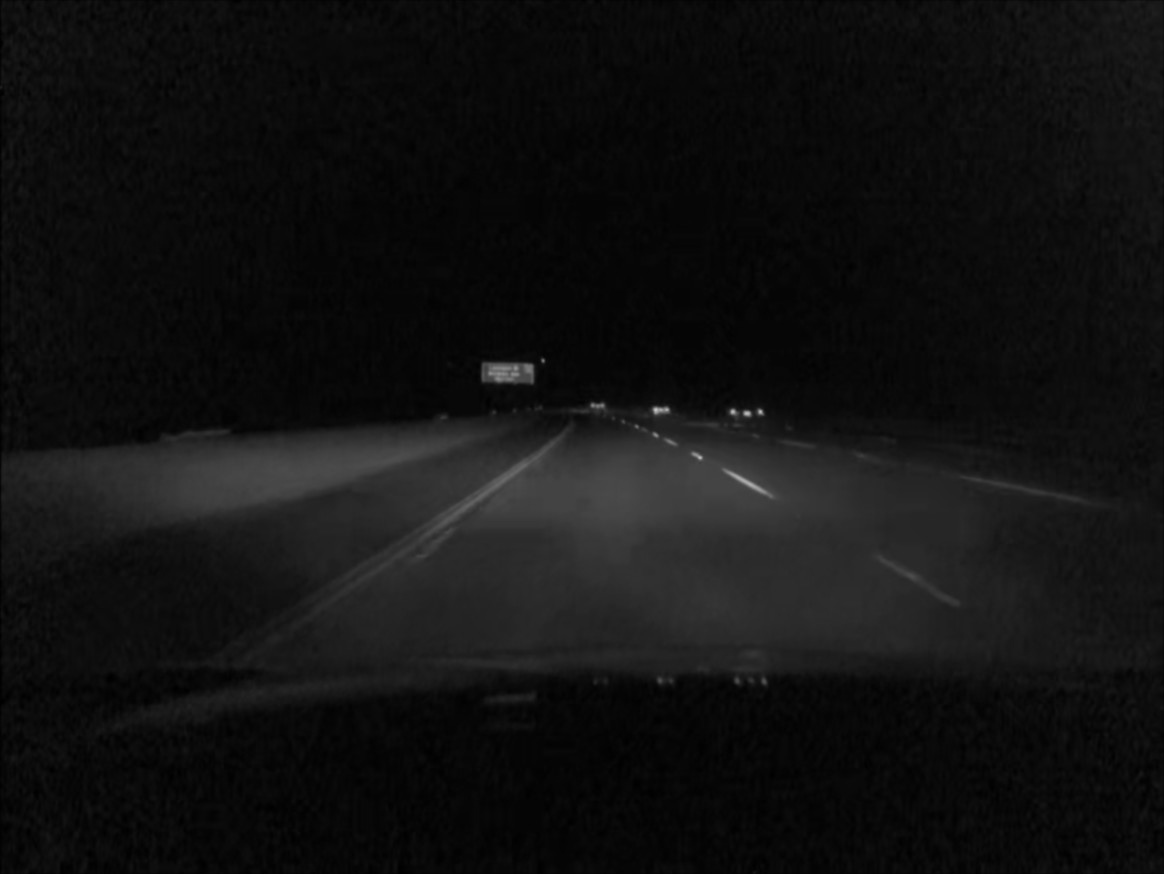
\includegraphics[height=6cm]{result_img/img1_q1.png}
  \caption{Image 1 : Gaussian Filter}
  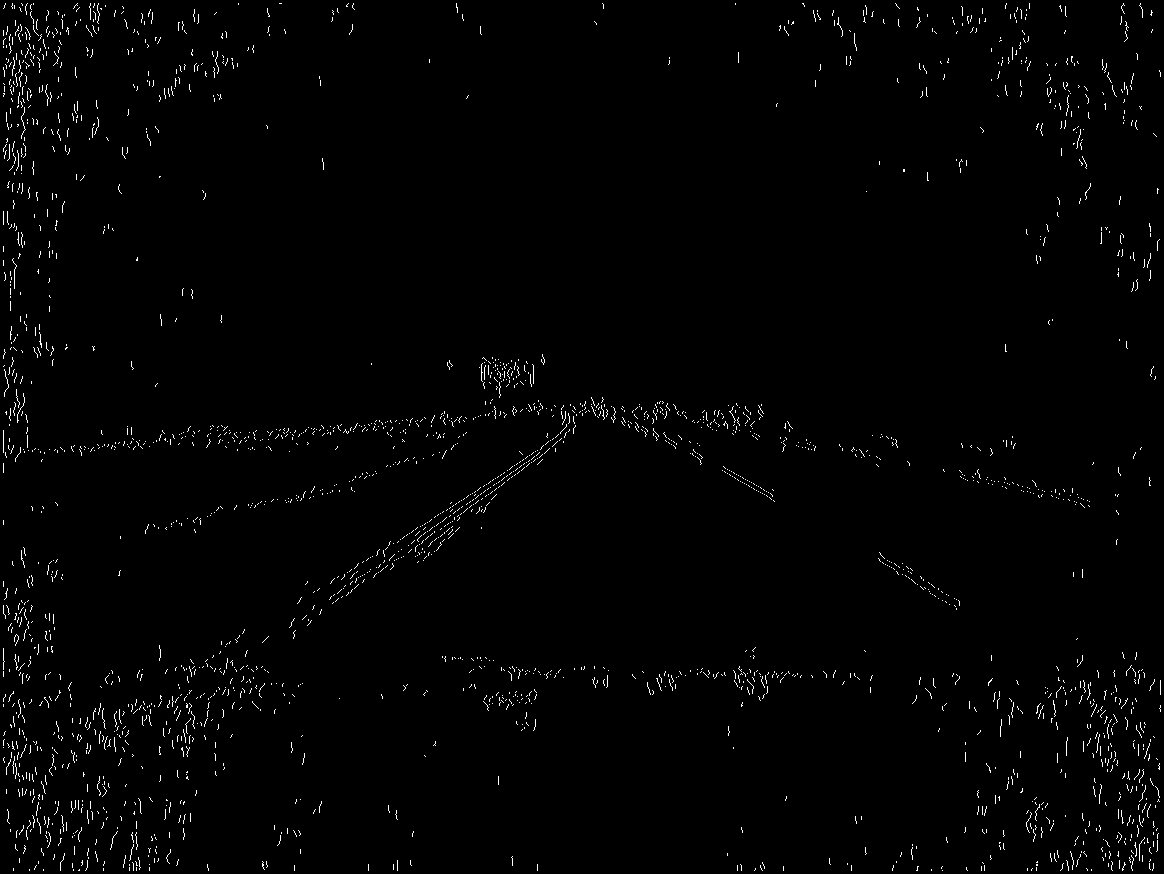
\includegraphics[height=6cm]{result_img/img1_q2.png}
  \caption{Image 1 : Canny Filter}
  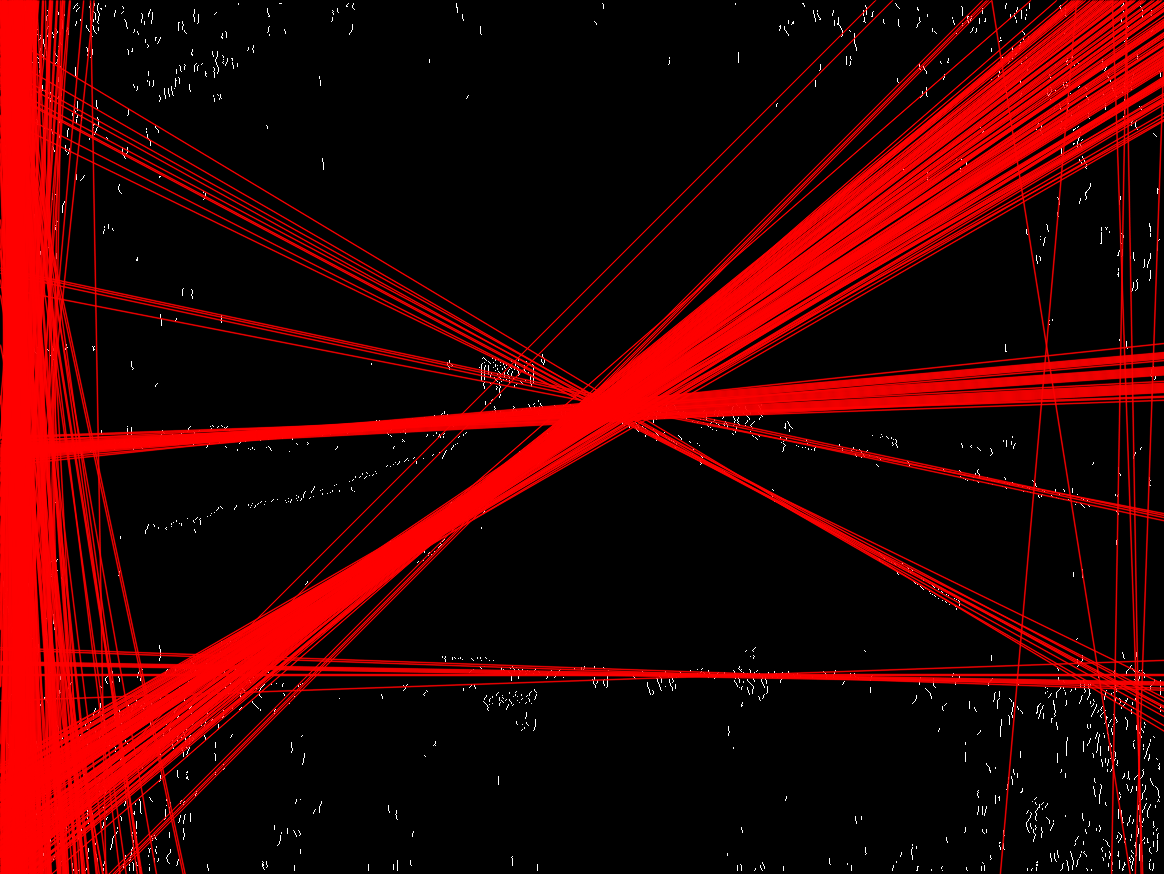
\includegraphics[height=6cm]{result_img/img1_q3.png}
  \caption{Image 1 : Hough Line Detector}
\end{figure}
\begin{figure}[!htb]
  \centering
  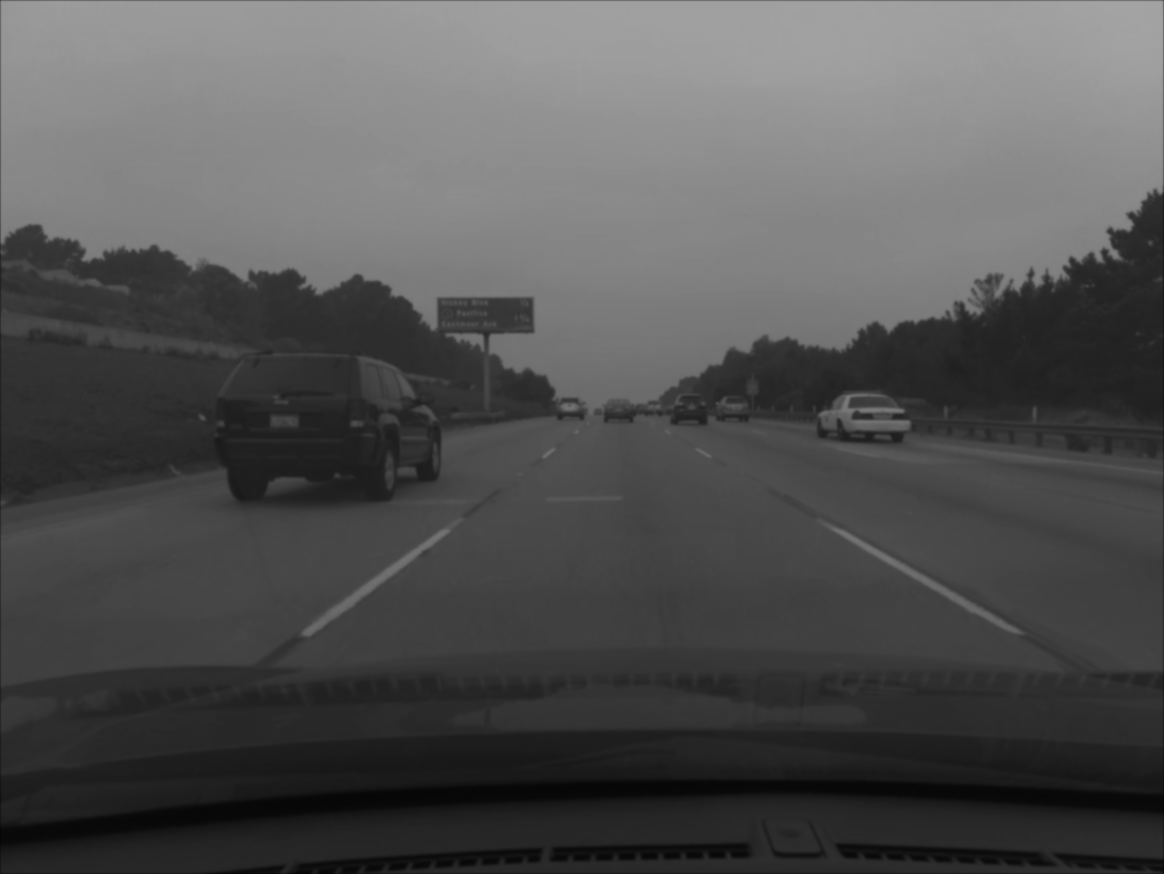
\includegraphics[height=6cm]{result_img/img2_q1.png}
  \caption{Image 2 : Gaussian Filter}
  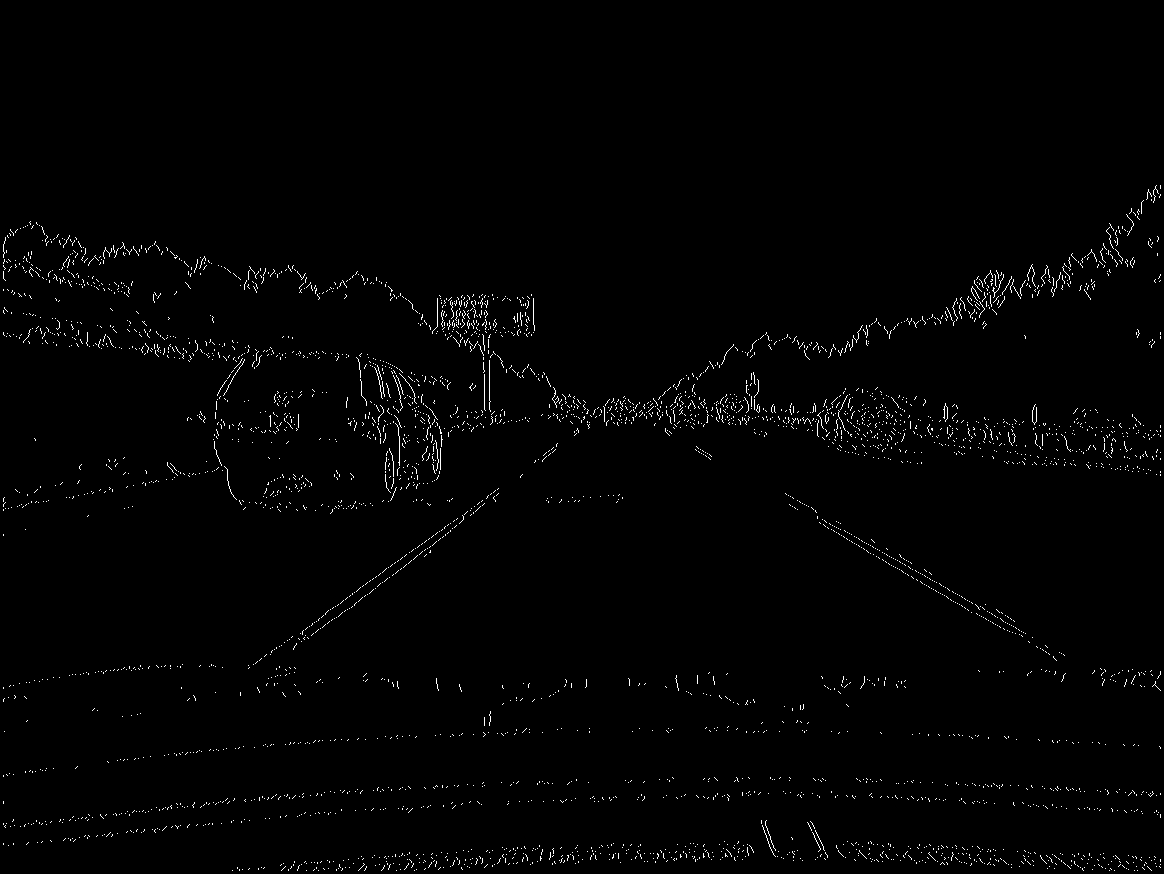
\includegraphics[height=6cm]{result_img/img2_q2.png}
  \caption{Image 2 : Canny Filter}
  \includegraphics[height=6cm]{result_img/img2_q3.png}
  \caption{Image 2 : Hough Line Detector}
\end{figure}
\begin{figure}[!htb]
  \centering
  \includegraphics[height=6cm]{result_img/img3_q1.png}
  \caption{Image 3 : Gaussian Filter}
  \includegraphics[height=6cm]{result_img/img3_q2.png}
  \caption{Image 3 : Canny Filter}
  \includegraphics[height=6cm]{result_img/img3_q3.png}
  \caption{Image 3 : Hough Line Detector}
\end{figure}
\end{document}
